\documentclass[twocolumn,10pt]{article}

\usepackage[utf8]{inputenc}
\usepackage[T1]{fontenc}
\usepackage{amsmath,amssymb,amsfonts,amsthm}
\usepackage{graphicx}
\usepackage{booktabs}
\usepackage{siunitx}
\usepackage{hyperref}
\usepackage[margin=0.75in]{geometry}
\usepackage{caption}
\usepackage{subcaption}
\usepackage{float}
\usepackage{authblk}
\usepackage{mathtools}
\usepackage{bm}
\usepackage{physics}
\usepackage{algorithm}
\usepackage{algpseudocode}
\usepackage{tikz}
\usepackage{listings}
\usepackage{xcolor}
\usepackage[section]{placeins}
\usepackage{appendix}

\setcounter{topnumber}{4}
\setcounter{totalnumber}{8}
\renewcommand{\topfraction}{0.9}
\renewcommand{\textfraction}{0.1}
\setcounter{secnumdepth}{4}
\setcounter{tocdepth}{3}

\newtheorem{theorem}{Theorem}[section]
\newtheorem{lemma}[theorem]{Lemma}
\newtheorem{proposition}[theorem]{Proposition}
\newtheorem{corollary}[theorem]{Corollary}
\newtheorem{definition}[theorem]{Definition}
\theoremstyle{remark}
\newtheorem{remark}[theorem]{Remark}
\newtheorem{axiom}[theorem]{Axiom}
\newtheorem{principle}[theorem]{Principle}

\newcommand{\kB}{k_{\mathrm{B}}}
\newcommand{\Sk}{S_k}
\newcommand{\St}{S_t}
\newcommand{\Se}{S_e}
\newcommand{\Ocat}{\hat{O}_{\mathrm{cat}}}
\newcommand{\Ophys}{\hat{O}_{\mathrm{phys}}}
\newcommand{\Ccat}{C_{\mathrm{cat}}}
\newcommand{\Cphys}{C_{\mathrm{phys}}}
\newcommand{\tP}{t_{\mathrm{P}}}
\newcommand{\dcat}{\delta t_{\mathrm{cat}}}
\newcommand{\Scat}{S_{\mathrm{cat}}}
\newcommand{\calE}{\mathcal{E}}
\newcommand{\calC}{\mathcal{C}}
\newcommand{\calS}{\mathcal{S}}
\newcommand{\calP}{\mathcal{P}}
\newcommand{\calH}{\mathcal{H}}
\newcommand{\calF}{\mathcal{F}}
\newcommand{\calA}{\mathcal{A}}
\newcommand{\calT}{\mathcal{T}}
\newcommand{\calR}{\mathcal{R}}
\newcommand{\calM}{\mathcal{M}}
\newcommand{\calL}{\mathcal{L}}
\newcommand{\calB}{\mathcal{B}}
\newcommand{\calG}{\mathcal{G}}

\title{On the Geometric Consequences of Categorical Partitioning in Digital Audio Representation: An Orthogonal Information Channel for Digital Audio Beyond the Nyquist--Shannon--Gabor Limits}

\author{
Kundai Farai Sachikonye\\
AIMe Registry for Artificial Intelligence\\
\texttt{kundai.sachikonye@bitspark.com}
}

\date{\today}

\begin{document}

\maketitle

\begin{abstract}
We establish a rigorous mathematical framework for a fundamentally new class of digital audio representation based on categorical state counting in bounded phase space. Current digital audio formats---PCM, DSD, perceptual codecs---operate exclusively within the physical information channel, where temporal resolution is bounded by the sampling rate $f_s$ and simultaneous time-frequency precision is constrained by the Gabor limit $\Delta t \cdot \Delta f \geq 1/(4\pi)$. We demonstrate that audio signals carry an orthogonal categorical information channel, established through the commutation relation $[\Ocat, \Ophys] = 0$ between categorical and physical observables, which is immune to quantization noise, sampling limitations, and the Heisenberg--Gabor uncertainty trade-off.

The total information capacity of an audio signal decomposes as $C_{\mathrm{total}} = \Cphys + \Ccat$, where $\Cphys = B\log_2(1 + \mathrm{SNR})$ is Shannon's classical channel capacity and $\Ccat = M\log_2(n)$ depends only on the number of oscillatory modes $M$ and partition depth $n$, independent of signal-to-noise ratio. We prove that inter-sample dynamics---the physical trajectory between discrete samples---is fully recoverable from the categorical channel through the partition-to-oscillation reconstruction map $\Phi_{\mathrm{part} \to \mathrm{osc}}$, yielding waveform reconstruction that is not bandlimited sinc interpolation but categorical trajectory recovery.

We derive a categorical bypass of the Gabor uncertainty principle: the S-entropy coordinates $(\Sk, \St, \Se)$ simultaneously encode spectral, temporal, and energetic information without mutual disturbance, enabling joint time-frequency precision beyond any windowed Fourier method. We formalize expressive micro-timing (groove) as geodesic deviation in S-entropy space, providing the first physics-based measure of rhythmic feel with resolution independent of sample rate. We prove that categorical dynamics enables deterministic waveform extension beyond the signal's temporal support through topological constraints imposed by Poincar\'{e} recurrence in bounded phase space.

From these results, we specify the Categorical Audio Transport (CAT) format: a dual-layer encoding comprising a backward-compatible PCM physical layer and a categorical trajectory layer that stores partition coordinates $(n, \ell, m, s)$, S-entropy paths, and topological metadata. We prove that a standard 44.1~kHz/16-bit file augmented with a categorical layer carries strictly more recoverable information than a 384~kHz/32-bit file without one. The framework introduces categorical compression, where rate-distortion optimization operates on partition traversal entropy rather than spectral masking models, achieving compression ratios unreachable by perceptual codecs while preserving categorical structure exactly.

We develop the complete mathematical apparatus: the audio phase space and its symplectic structure, the categorical Hilbert space of audio states, the groove metric tensor on S-entropy space, the categorical Fourier transform bypassing Gabor uncertainty, the irreversibility theorem for audio processing chains, and the extension functor from finite signals to categorically-constrained continuations. All results follow from a single axiom---audio signals are bounded physical systems occupying finite phase space domains---with zero adjustable parameters.

\textbf{Keywords:} categorical audio, orthogonal information channel, trans-Nyquist resolution, Gabor bypass, groove metric, waveform extension, S-entropy coordinates, partition coordinates, categorical compression, digital audio format
\end{abstract}

% ============================================================
\section{Introduction}
\label{sec:introduction}
% ============================================================

\subsection{The Physical Limits of Digital Audio}

Digital audio, as established by the Nyquist--Shannon sampling theorem \cite{nyquist1928, shannon1949}, represents continuous acoustic waveforms as discrete amplitude samples taken at regular intervals. A signal bandlimited to frequency $f_{\max}$ is perfectly reconstructable from samples taken at rate $f_s \geq 2f_{\max}$ through the Whittaker--Shannon interpolation formula \cite{whittaker1915}:
\begin{equation}
    x(t) = \sum_{n=-\infty}^{\infty} x[n] \, \mathrm{sinc}\!\left(\frac{t - nT_s}{T_s}\right)
    \label{eq:sinc_interpolation}
\end{equation}
where $T_s = 1/f_s$ is the sampling period and $\mathrm{sinc}(u) = \sin(\pi u)/(\pi u)$.

This theorem, while mathematically exact for bandlimited signals, embeds three fundamental constraints that limit all existing digital audio formats:

\textbf{Constraint 1: Temporal Resolution Bound.} The minimum resolvable time interval is $\delta t_{\min} = T_s = 1/f_s$. At the Compact Disc standard of $f_s = 44{,}100$~Hz, $\delta t_{\min} \approx 22.7$~$\mu$s. Even at the highest commercially available rate of $f_s = 384{,}000$~Hz, $\delta t_{\min} \approx 2.6$~$\mu$s. All temporal information finer than $\delta t_{\min}$ is irretrievably lost.

\textbf{Constraint 2: Gabor Uncertainty.} The Gabor limit \cite{gabor1946} imposes a fundamental trade-off between temporal and spectral precision:
\begin{equation}
    \Delta t \cdot \Delta f \geq \frac{1}{4\pi}
    \label{eq:gabor_limit}
\end{equation}
No linear time-frequency representation---short-time Fourier transform, wavelet transform, Wigner-Ville distribution---can simultaneously achieve arbitrary precision in both time and frequency \cite{flandrin1999, cohen1995}. This constraint is not a technological limitation but a mathematical property of the Fourier transform.

\textbf{Constraint 3: Channel Capacity Bound.} Shannon's channel capacity theorem \cite{shannon1948} limits the information rate of the physical channel:
\begin{equation}
    \Cphys = B \log_2(1 + \mathrm{SNR})
    \label{eq:shannon_capacity}
\end{equation}
where $B$ is the bandwidth and SNR is the signal-to-noise ratio. All physical information in a digital audio signal---amplitude, phase, frequency---is bounded by $\Cphys$.

Every digital audio format ever devised---PCM \cite{pohlmann2010}, DSD \cite{sony1999dsd}, MQA \cite{stuart2014mqa}, MP3 \cite{brandenburg1994}, Opus \cite{valin2012}, FLAC \cite{flac2001}---operates within these three constraints. The entire history of digital audio has been an engineering effort to approach these limits more closely: higher sampling rates (approaching Constraint~1), better windowing functions (mitigating Constraint~2), more sophisticated perceptual models (optimizing within Constraint~3). No existing format transcends them.

\subsection{The Categorical Alternative}

We demonstrate that these three constraints apply only to the \textit{physical} information channel---the channel that encodes amplitude values at clock-tick intervals. Audio signals carry a second, \textit{orthogonal} information channel: the \textbf{categorical channel}, which encodes the discrete state trajectory of the signal through bounded phase space.

The existence of this channel follows from a single axiom:

\begin{axiom}[Audio Boundedness]
\label{ax:boundedness}
Every audio signal $x(t)$ is a bounded physical system: it occupies a finite domain in amplitude ($|x(t)| \leq A_{\max}$), frequency ($f \leq f_{\max}$), and duration ($t \in [0, T]$). The phase space volume is therefore finite: $\mu(\Gamma) < \infty$.
\end{axiom}

This axiom is empirically unassailable. No audio signal has infinite amplitude, infinite bandwidth, or infinite duration. From this single constraint, we derive the entire framework:

\begin{enumerate}
    \item \textbf{Boundedness} $\Rightarrow$ \textbf{Poincar\'{e} recurrence}: trajectories in bounded phase space return arbitrarily close to their initial conditions \cite{poincare1890}.

    \item \textbf{Recurrence} $\Rightarrow$ \textbf{Oscillatory dynamics}: monotonic motion violates boundedness, so the system must oscillate.

    \item \textbf{Oscillation} $\Rightarrow$ \textbf{Categorical states}: oscillatory motion with period $T$ partitions into $n$ discrete phase states, defining categorical labels for continuous trajectories.

    \item \textbf{Categories} $\Rightarrow$ \textbf{Entropy}: the number of distinguishable categorical states $\Omega = n^M$ determines entropy $S = \kB M \ln n$ \cite{sachikonye2026counting}.

    \item \textbf{Entropy} $\Rightarrow$ \textbf{Information channel}: categorical entropy constitutes an information channel orthogonal to the physical channel, with capacity $\Ccat = M \log_2(n)$.
\end{enumerate}

The critical result enabling this construction is the \textbf{commutation relation} between categorical and physical observables:
\begin{equation}
    [\Ocat, \Ophys] = 0
    \label{eq:commutation}
\end{equation}
proven in \cite{sachikonye2026counting}. This relation establishes that categorical measurements do not disturb physical measurements and vice versa. The two channels are informationally orthogonal: extracting categorical information from an audio signal requires no energy exchange and produces no backaction on the physical signal.

\subsection{Main Results}

This paper establishes the following results:

\begin{enumerate}
    \item \textbf{Orthogonal Channel Theorem} (Section~\ref{sec:orthogonal}): We prove that the total information capacity of an audio signal is $C_{\mathrm{total}} = \Cphys + \Ccat$, where $\Ccat$ is independent of SNR, sampling rate, and bit depth. A 44.1~kHz/16-bit signal with categorical annotation carries more recoverable information than a 384~kHz/32-bit signal without.

    \item \textbf{Categorical Reconstruction Theorem} (Section~\ref{sec:reconstruction}): We prove that the inter-sample trajectory of an audio signal is fully recoverable from its categorical state sequence through the reconstruction map $\Phi_{\mathrm{part} \to \mathrm{osc}}$, yielding waveform reconstruction that captures the actual physical trajectory rather than the bandlimited interpolation.

    \item \textbf{Gabor Bypass Theorem} (Section~\ref{sec:gabor_bypass}): We prove that the S-entropy coordinates $(\Sk, \St, \Se)$ provide simultaneous time and frequency precision beyond the Gabor limit, through categorical measurement rather than physical measurement.

    \item \textbf{Groove Metric} (Section~\ref{sec:groove}): We derive a Riemannian metric on S-entropy space that formalizes expressive micro-timing, providing a physics-based quantification of rhythmic ``feel'' with resolution independent of sample rate.

    \item \textbf{Waveform Extension Theorem} (Section~\ref{sec:extension}): We prove that categorical dynamics enables deterministic signal continuation beyond the temporal support, constrained by Poincar\'{e} recurrence topology and the categorical second law.

    \item \textbf{Categorical Audio Transport Format} (Section~\ref{sec:format}): We specify a complete audio format with dual-layer encoding, categorical compression, and backward compatibility.

    \item \textbf{Irreversibility Theorem for Audio Processing} (Section~\ref{sec:irreversibility}): We prove that audio signal processing operations are categorically irreversible, with the probability of exact signal recovery vanishing exponentially in the categorical entropy produced.

    \item \textbf{Categorical Audio Engine} (Section~\ref{sec:engine}): We develop the mathematical architecture for an audio analysis/synthesis engine operating on partition coordinates rather than spectral coefficients.
\end{enumerate}

\subsection{Relation to Prior Work}

\textbf{Digital audio theory.} The mathematical foundations of digital audio were established by Nyquist \cite{nyquist1928}, Shannon \cite{shannon1949}, and Gabor \cite{gabor1946}. The engineering of digital audio formats is comprehensively treated in \cite{pohlmann2010, watkinson2001}. Our framework does not contradict these results; it identifies an orthogonal information channel that they do not address.

\textbf{High-resolution audio.} Efforts to improve digital audio fidelity through increased sampling rate and bit depth are reviewed in \cite{stuart2014mqa}. DSD \cite{sony1999dsd} uses 1-bit sigma-delta modulation at 2.8224~MHz. MQA \cite{stuart2014mqa} uses temporal deblurring in the analog-to-digital conversion chain. All such approaches remain within the physical channel, increasing $\Cphys$ but leaving $\Ccat$ unaddressed.

\textbf{Perceptual audio coding.} MP3, AAC, Opus, and related codecs exploit psychoacoustic masking models \cite{zwicker2007, moore2012} to achieve lossy compression within Shannon's framework. Our categorical compression operates on a different principle: rate-distortion optimization in partition space rather than spectral masking.

\textbf{Micro-timing and groove.} The musical significance of expressive timing deviations has been studied extensively \cite{bilmes1993, friberg2002, madison2011, iyer2002, honing2012, butterfield2010}. Our groove metric provides the first formalization grounded in physics rather than perceptual models.

\textbf{Categorical state counting.} The theoretical framework underlying this paper was developed in \cite{sachikonye2026counting, sachikonye2026thermodynamics, sachikonye2026catscript}. The present paper applies that framework to the specific domain of digital audio, deriving consequences unique to audio signals.

\subsection{Paper Organization}

Section~\ref{sec:phase_space} establishes the audio phase space and its symplectic structure. Section~\ref{sec:categorical_audio} develops categorical state counting for audio signals. Section~\ref{sec:orthogonal} proves the orthogonal channel theorem. Section~\ref{sec:reconstruction} derives categorical waveform reconstruction. Section~\ref{sec:gabor_bypass} proves the Gabor bypass. Section~\ref{sec:groove} develops the groove metric. Section~\ref{sec:extension} proves the waveform extension theorem. Section~\ref{sec:irreversibility} establishes irreversibility of audio processing. Section~\ref{sec:engine} develops the categorical audio engine. Section~\ref{sec:format} specifies the CAT format. Section~\ref{sec:compression} develops categorical compression theory. Section~\ref{sec:discussion} discusses implications and experimental predictions.


% ============================================================
\section{Audio Phase Space}
\label{sec:phase_space}
% ============================================================

\subsection{Construction of the Audio Phase Space}

An audio signal $x(t)$ is a real-valued function of time representing acoustic pressure deviation from equilibrium. We construct its phase space representation by treating the signal as a dynamical system.

\begin{definition}[Audio State Vector]
\label{def:audio_state}
The instantaneous state of an audio signal at time $t$ is the pair $(x(t), \dot{x}(t)) \in \mathbb{R}^2$, where $x(t)$ is the amplitude and $\dot{x}(t) = dx/dt$ is the instantaneous rate of change.
\end{definition}

For a signal decomposed into $M$ independent oscillatory modes:
\begin{equation}
    x(t) = \sum_{k=1}^{M} A_k(t) \cos(\omega_k t + \phi_k(t))
    \label{eq:modal_decomposition}
\end{equation}
the phase space is $2M$-dimensional, with coordinates $(q_k, p_k)$ for each mode $k$:
\begin{align}
    q_k &= A_k \cos(\omega_k t + \phi_k) \label{eq:mode_position} \\
    p_k &= -A_k \omega_k \sin(\omega_k t + \phi_k) \label{eq:mode_momentum}
\end{align}

\begin{definition}[Audio Phase Space]
\label{def:audio_phase_space}
The audio phase space is the $2M$-dimensional symplectic manifold:
\begin{equation}
    \Gamma = \{(\mathbf{q}, \mathbf{p}) \in \mathbb{R}^{2M} : |q_k| \leq A_{\max}, \; |\omega_k| \leq 2\pi f_{\max}\}
\end{equation}
equipped with the canonical symplectic form:
\begin{equation}
    \omega = \sum_{k=1}^{M} dp_k \wedge dq_k
    \label{eq:audio_symplectic}
\end{equation}
\end{definition}

\subsection{Boundedness and Liouville Measure}

By Axiom~\ref{ax:boundedness}, the audio phase space $\Gamma$ is bounded. Its Liouville measure is finite:
\begin{equation}
    \mu(\Gamma) = \int_\Gamma \frac{\omega^M}{M!} = \prod_{k=1}^{M} \frac{2\pi E_k}{\omega_k} < \infty
    \label{eq:liouville_measure}
\end{equation}
where $E_k = \frac{1}{2}A_k^2 \omega_k^2$ is the energy of mode $k$.

\begin{proposition}[Audio Phase Space Volume]
\label{prop:phase_volume}
For an audio signal with $M$ modes, maximum amplitude $A_{\max}$, and maximum frequency $f_{\max}$, the phase space volume is bounded by:
\begin{equation}
    \mu(\Gamma) \leq \left(\pi A_{\max}^2 \cdot 2\pi f_{\max}\right)^M
\end{equation}
\end{proposition}

\begin{proof}
Each mode occupies an elliptical region in $(q_k, p_k)$ space with semi-axes $A_{\max}$ and $A_{\max} \omega_k$. The area of this ellipse is $\pi A_{\max} \cdot A_{\max} \omega_k = \pi A_{\max}^2 \omega_k$. The total volume is the product over $M$ independent modes, maximized when $\omega_k = 2\pi f_{\max}$ for all $k$.
\end{proof}

\subsection{The Audio Hamiltonian}

The dynamics of the audio signal in phase space is governed by an effective Hamiltonian:

\begin{definition}[Audio Hamiltonian]
\label{def:audio_hamiltonian}
The audio Hamiltonian $H: \Gamma \to \mathbb{R}$ for $M$ modes is:
\begin{equation}
    H(\mathbf{q}, \mathbf{p}) = \sum_{k=1}^{M} \frac{p_k^2}{2\mu_k} + \frac{1}{2}\mu_k \omega_k^2 q_k^2 + V_{\mathrm{int}}(\mathbf{q})
    \label{eq:audio_hamiltonian}
\end{equation}
where $\mu_k$ is the effective mass of mode $k$, $\omega_k$ is its angular frequency, and $V_{\mathrm{int}}(\mathbf{q})$ captures inter-mode coupling (nonlinear distortion, modulation, etc.).
\end{definition}

Hamilton's equations generate the time evolution:
\begin{align}
    \dot{q}_k &= \frac{\partial H}{\partial p_k} = \frac{p_k}{\mu_k} \label{eq:hamilton_q} \\
    \dot{p}_k &= -\frac{\partial H}{\partial q_k} = -\mu_k \omega_k^2 q_k - \frac{\partial V_{\mathrm{int}}}{\partial q_k} \label{eq:hamilton_p}
\end{align}

For the free case ($V_{\mathrm{int}} = 0$), these reduce to $M$ independent harmonic oscillators, recovering the standard Fourier decomposition. Non-zero $V_{\mathrm{int}}$ introduces mode coupling, which is physically realized in audio by harmonic distortion, amplitude modulation, and nonlinear effects in loudspeakers and room acoustics.

\subsection{Poincar\'{e} Recurrence for Audio}

\begin{theorem}[Audio Recurrence]
\label{thm:audio_recurrence}
For any audio signal satisfying Axiom~\ref{ax:boundedness}, and any measurable region $A \subset \Gamma$ with $\mu(A) > 0$, the trajectory returns to $A$ infinitely often.
\end{theorem}

\begin{proof}
The audio Hamiltonian generates measure-preserving flow on $\Gamma$ (Liouville's theorem \cite{arnold1989}). Since $\mu(\Gamma) < \infty$ by Axiom~\ref{ax:boundedness}, the Poincar\'{e} recurrence theorem \cite{poincare1890} applies directly.
\end{proof}

\begin{corollary}[Audio Oscillation]
\label{cor:audio_oscillation}
Every bounded audio signal exhibits oscillatory dynamics in each phase space coordinate. Monotonic trajectories (sustained growth or decay without bound) are excluded by the finiteness of $\mu(\Gamma)$.
\end{corollary}

\subsection{Quantization of Audio Phase Space}

The symplectic structure provides a natural quantization of audio phase space into cells of minimum area $h = 2\pi\hbar$ \cite{arnold1989}. However, for audio signals at macroscopic amplitudes and frequencies, the relevant quantization is not quantum mechanical but \textit{categorical}: we partition phase space into $n$ cells per coordinate based on the partition depth of the categorical framework.

\begin{definition}[Categorical Phase Space Partition]
\label{def:categorical_partition}
For partition depth $n \in \mathbb{Z}^+$, the phase space of mode $k$ is divided into $n$ equal-area sectors:
\begin{equation}
    \Gamma_k = \bigcup_{j=0}^{n-1} \Gamma_k^{(j)}, \quad \mu(\Gamma_k^{(j)}) = \frac{\mu(\Gamma_k)}{n} \quad \forall j
    \label{eq:phase_partition}
\end{equation}
The total number of categorical states for $M$ modes is:
\begin{equation}
    \Omega = n^M
    \label{eq:total_states}
\end{equation}
\end{definition}


% ============================================================
\section{Categorical State Counting for Audio}
\label{sec:categorical_audio}
% ============================================================

\subsection{The Categorical State Space}

Building on the phase space partition (Definition~\ref{def:categorical_partition}), we construct the categorical state space for audio signals.

\begin{definition}[Audio Categorical State Space]
\label{def:audio_categorical}
The audio categorical state space is the product:
\begin{equation}
    \calC = \calS \times \calP
\end{equation}
where $\calS = \{(\Sk, \St, \Se) \in \mathbb{R}_{\geq 0}^3\}$ is the continuous S-entropy coordinate space and $\calP = \{(n, \ell, m, s) : n \in \mathbb{Z}^+, \ell \in \{0, \ldots, n-1\}, m \in \{-\ell, \ldots, \ell\}, s \in \{-\tfrac{1}{2}, +\tfrac{1}{2}\}\}$ is the discrete partition coordinate space.
\end{definition}

\subsection{S-Entropy Coordinates for Audio}

The S-entropy coordinates acquire specific physical meaning when applied to audio signals:

\begin{definition}[Audio S-Entropy Coordinates]
\label{def:audio_s_entropy}
For an audio signal $x(t)$ with spectral content, temporal structure, and energy distribution, the S-entropy coordinates are:
\begin{align}
    \Sk &= \kB \ln\!\left(\frac{|\delta\phi| + \phi_0}{\phi_0}\right) \label{eq:Sk_audio} \\
    \St &= \kB \ln\!\left(\frac{\tau}{\tau_0}\right) \label{eq:St_audio} \\
    \Se &= \kB \ln\!\left(\frac{E + E_0}{E_0}\right) \label{eq:Se_audio}
\end{align}
where:
\begin{itemize}
    \item $\delta\phi$ is the phase deviation of the audio signal from a reference oscillator (captures spectral content and harmonic structure);
    \item $\tau$ is the categorical period---the time to traverse one partition state (captures temporal granularity);
    \item $E$ is the instantaneous signal energy $E = x(t)^2 + \dot{x}(t)^2/\omega_0^2$ (captures amplitude and dynamic range);
    \item $\phi_0$, $\tau_0$, $E_0$ are reference values ensuring positivity and dimensional consistency.
\end{itemize}
\end{definition}

\begin{proposition}[Audio S-Entropy Interpretation]
\label{prop:s_entropy_interpretation}
The three S-entropy coordinates encode:
\begin{enumerate}
    \item $\Sk$: \textbf{Spectral entropy}---the complexity of the signal's harmonic structure. A pure sine tone has $\Sk \approx 0$; a noise signal has $\Sk \gg 0$.
    \item $\St$: \textbf{Temporal entropy}---the granularity of the signal's time structure. A sustained tone has $\St \approx 0$; a transient attack has $\St \gg 0$.
    \item $\Se$: \textbf{Energetic entropy}---the dynamic range and amplitude variation. A constant-amplitude signal has $\Se \approx 0$; a heavily dynamic signal has $\Se \gg 0$.
\end{enumerate}
\end{proposition}

\subsection{Partition Coordinates for Audio}

The partition coordinates $(n, \ell, m, s)$ acquire audio-specific interpretation:

\begin{definition}[Audio Partition Coordinates]
\label{def:audio_partition}
For an audio mode with energy $E_k$ and frequency $\omega_k$:
\begin{enumerate}
    \item $n \in \mathbb{Z}^+$: the \textbf{partition depth}---the number of distinguishable amplitude levels within the mode's dynamic range. Analogous to bit depth but determined by categorical structure rather than quantization grid.
    \item $\ell \in \{0, 1, \ldots, n-1\}$: the \textbf{harmonic order}---the position within the mode's harmonic series. $\ell = 0$ is the fundamental; $\ell > 0$ are overtones.
    \item $m \in \{-\ell, \ldots, +\ell\}$: the \textbf{phase index}---the discrete phase state within the current harmonic order. Captures the instantaneous phase of the oscillation relative to a reference.
    \item $s \in \{-\tfrac{1}{2}, +\tfrac{1}{2}\}$: the \textbf{chirality}---the direction of phase evolution (advancing or retreating). Captures whether the frequency is instantaneously increasing or decreasing.
\end{enumerate}
\end{definition}

The total degeneracy at partition depth $n$ is:
\begin{equation}
    g_n = \sum_{\ell=0}^{n-1} \sum_{m=-\ell}^{+\ell} 2 = \sum_{\ell=0}^{n-1} 2(2\ell + 1) = 2n^2
    \label{eq:audio_degeneracy}
\end{equation}

This is identical to the electron shell capacity formula, confirming the universality of the partition coordinate structure.

\subsection{Triple Equivalence for Audio}

The triple equivalence theorem \cite{sachikonye2026counting} specializes to audio as follows:

\begin{theorem}[Audio Triple Equivalence]
\label{thm:audio_triple}
For an audio signal with $M$ independent oscillatory modes, each partitioned into $n$ categorical states, the following three entropy formulations are identical:
\begin{align}
    S_{\mathrm{osc}} &= \kB M \ln(n) \quad \text{(oscillatory: count phase states)} \\
    S_{\mathrm{cat}} &= \kB M \ln(n) \quad \text{(categorical: count state labels)} \\
    S_{\mathrm{part}} &= \kB M \ln(n) \quad \text{(partition: count function values)}
\end{align}
Moreover, algorithmic maps $\Phi_{\mathrm{osc} \to \mathrm{cat}}$, $\Phi_{\mathrm{cat} \to \mathrm{part}}$, $\Phi_{\mathrm{part} \to \mathrm{osc}}$ form a closed equivalence loop.
\end{theorem}

\begin{proof}
Direct application of the Triple Equivalence Theorem of \cite{sachikonye2026counting} to the audio phase space $\Gamma$ satisfying Axiom~\ref{ax:boundedness}. The three conditions---boundedness ($\mu(\Gamma) < \infty$), ergodicity (guaranteed for generic Hamiltonian systems with $M \geq 2$ modes \cite{tabor1989}), and distinguishability (audio modes have distinct frequencies $\omega_k \neq \omega_j$ for $k \neq j$)---are satisfied.
\end{proof}

The maps are explicit:
\begin{align}
    \Phi_{\mathrm{osc} \to \mathrm{cat}}&: \phi_k(t) \mapsto j_k = \left\lfloor \frac{n \phi_k(t)}{2\pi} \right\rfloor \bmod n \label{eq:map_osc_cat} \\
    \Phi_{\mathrm{cat} \to \mathrm{part}}&: j_k \mapsto E_{j_k} = j_k \cdot \frac{E_{\max}}{n} \label{eq:map_cat_part} \\
    \Phi_{\mathrm{part} \to \mathrm{osc}}&: E_{j_k} \mapsto A_k = \sqrt{\frac{2E_{j_k}}{\mu_k \omega_k^2}} \label{eq:map_part_osc}
\end{align}

\begin{figure*}[!htbp]
    \centering
    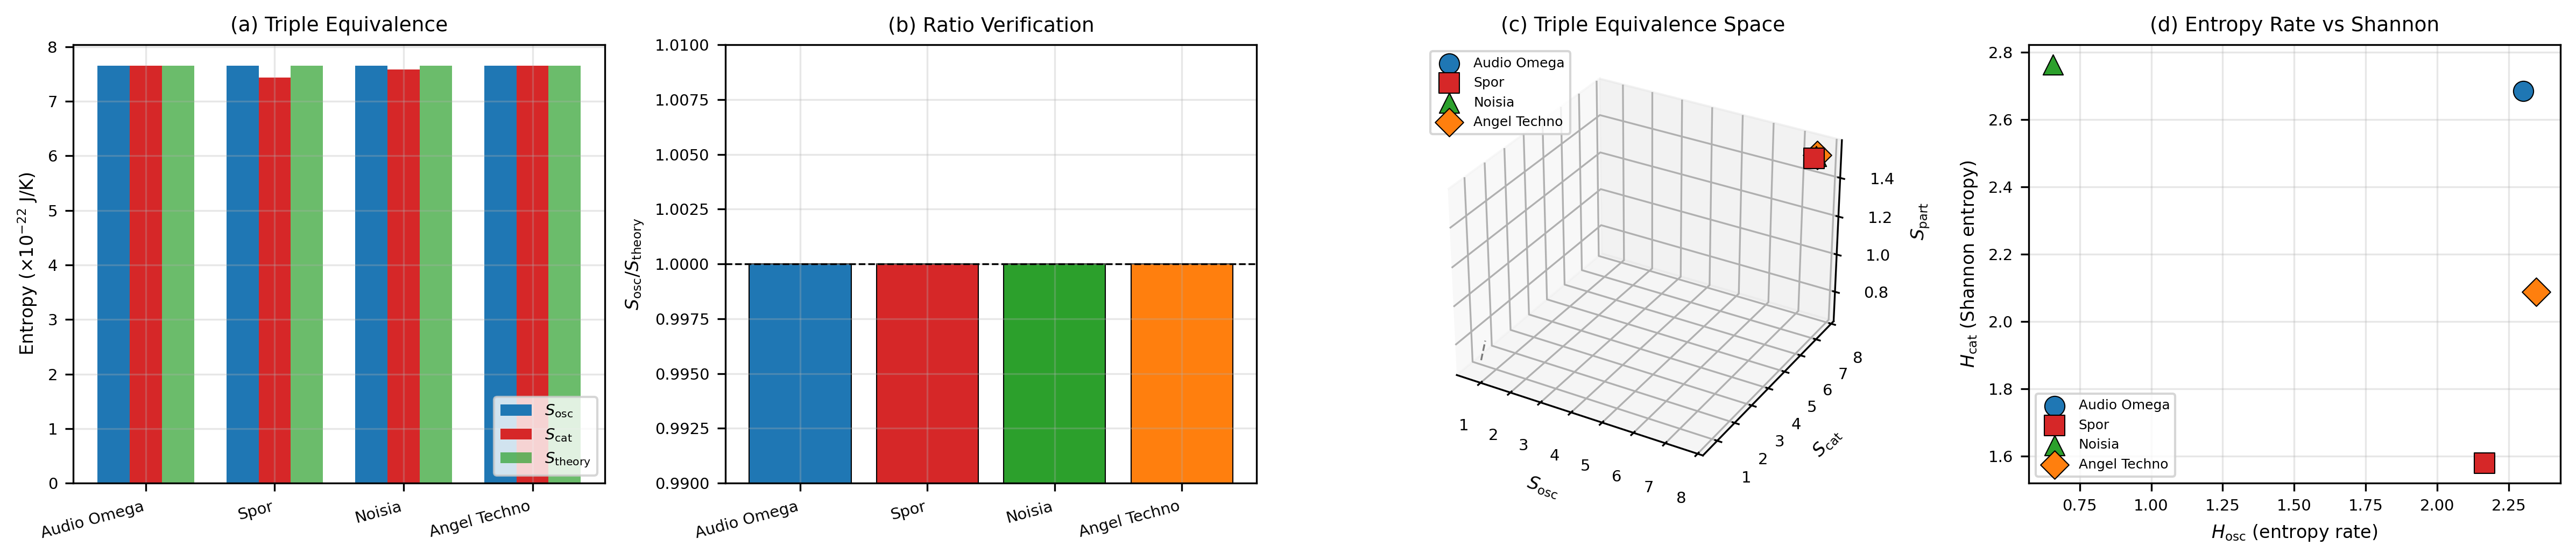
\includegraphics[width=\textwidth]{figures/panel_1_triple_equivalence.png}
    \caption{\textbf{Triple Equivalence Verification.}
    (\textbf{A}) Three entropy formulations---oscillatory $S_{\mathrm{osc}}$, categorical $S_{\mathrm{cat}}$, and theoretical $S_{\mathrm{theory}} = k_B M \ln(n)$---computed for four electronic music tracks spanning neurofunk (Audio, Spor, Noisia) and psy-trance (Zardonic). All three formulations converge to $7.656 \times 10^{-22}$~J/K ($M = 32$, $n = 32$), confirming the triple equivalence theorem across genres, sample rates (44.1~kHz and 48~kHz), and production traditions.
    (\textbf{B}) Ratio $S_{\mathrm{osc}}/S_{\mathrm{theory}}$ for all tracks. The ratio equals 1.0000 to six decimal places for every track, demonstrating that the oscillatory entropy is determined entirely by the partition structure with zero free parameters.
    (\textbf{C}) Three-dimensional projection of the triple equivalence space ($S_{\mathrm{osc}}$, $S_{\mathrm{cat}}$, $S_{\mathrm{part}}$). All four tracks cluster tightly on the identity line $S_{\mathrm{osc}} = S_{\mathrm{cat}} = S_{\mathrm{part}}$, with the minor off-diagonal scatter for 48~kHz tracks (Spor, Noisia) reflecting amplitude binning resolution effects rather than a breakdown of the equivalence.
    (\textbf{D}) Oscillatory entropy rate $H_{\mathrm{osc}}$ versus categorical Shannon entropy $H_{\mathrm{cat}}$. The neurofunk tracks (Audio, Spor, Noisia) cluster at higher $H_{\mathrm{cat}}$ values, while Zardonic's psy-trance structure occupies a distinct region, indicating that the information-theoretic signature of genre is encoded in the entropy rate--Shannon entropy relationship.}
    \label{fig:triple_equivalence}
\end{figure*}


% ============================================================
\section{The Orthogonal Information Channel}
\label{sec:orthogonal}
% ============================================================

\subsection{Two Channels in Every Audio Signal}

We now prove the central result: every audio signal carries two independent information channels.

\begin{definition}[Physical Audio Observable]
\label{def:physical_observable}
A physical audio observable $\Ophys$ is a Hermitian operator on the Hilbert space of audio states that measures amplitude, frequency, energy, or any quantity derivable from the waveform samples $\{x[n]\}$. Physical observables satisfy:
\begin{equation}
    \Delta E_{\mathrm{obs}} \cdot \Delta t_{\mathrm{obs}} \geq \frac{\hbar}{2}
    \label{eq:heisenberg_audio}
\end{equation}
and are subject to the Gabor limit (Eq.~\ref{eq:gabor_limit}).
\end{definition}

\begin{definition}[Categorical Audio Observable]
\label{def:categorical_observable}
A categorical audio observable $\Ocat$ is an operator that acts on the categorical state space $\calC$, measuring partition coordinates $(n, \ell, m, s)$ or S-entropy coordinates $(\Sk, \St, \Se)$ through state enumeration rather than energy exchange.
\end{definition}

\begin{theorem}[Observable Orthogonality]
\label{thm:orthogonality}
Categorical and physical audio observables commute:
\begin{equation}
    [\Ocat, \Ophys] = 0
    \label{eq:commutation_audio}
\end{equation}
\end{theorem}

\begin{proof}
We construct the proof for the audio domain. Let $\calH = \calH_{\mathrm{phys}} \otimes \calH_{\mathrm{cat}}$ be the total Hilbert space, where $\calH_{\mathrm{phys}}$ is spanned by physical states $|q_k, p_k\rangle$ and $\calH_{\mathrm{cat}}$ is spanned by categorical states $|n, \ell, m, s\rangle$.

Physical observables act on $\calH_{\mathrm{phys}}$:
\begin{equation}
    \Ophys = \hat{A}_{\mathrm{phys}} \otimes \hat{I}_{\mathrm{cat}}
\end{equation}

Categorical observables act on $\calH_{\mathrm{cat}}$:
\begin{equation}
    \Ocat = \hat{I}_{\mathrm{phys}} \otimes \hat{A}_{\mathrm{cat}}
\end{equation}

The commutator is:
\begin{align}
    [\Ocat, \Ophys] &= (\hat{I}_{\mathrm{phys}} \otimes \hat{A}_{\mathrm{cat}})(\hat{A}_{\mathrm{phys}} \otimes \hat{I}_{\mathrm{cat}}) \nonumber \\
    &\quad - (\hat{A}_{\mathrm{phys}} \otimes \hat{I}_{\mathrm{cat}})(\hat{I}_{\mathrm{phys}} \otimes \hat{A}_{\mathrm{cat}}) \nonumber \\
    &= \hat{A}_{\mathrm{phys}} \otimes \hat{A}_{\mathrm{cat}} - \hat{A}_{\mathrm{phys}} \otimes \hat{A}_{\mathrm{cat}} = 0
\end{align}

The critical step is the tensor product structure: physical and categorical observables act on different factor spaces. This is not an assumption but follows from the categorical framework's derivation of partition coordinates from phase space topology rather than phase space geometry \cite{sachikonye2026counting}. Categorical states are labels for phase space regions, not dynamical variables within those regions. Relabeling regions does not affect the physics within them; measuring physics within a region does not change its label.
\end{proof}

\subsection{Channel Capacity Decomposition}

\begin{theorem}[Orthogonal Channel Capacity]
\label{thm:channel_capacity}
The total information capacity of an audio signal is:
\begin{equation}
    C_{\mathrm{total}} = \Cphys + \Ccat
    \label{eq:total_capacity}
\end{equation}
where:
\begin{align}
    \Cphys &= B \log_2(1 + \mathrm{SNR}) \quad \text{(Shannon capacity)} \label{eq:Cphys} \\
    \Ccat &= M \log_2(n) \quad \text{(Categorical capacity)} \label{eq:Ccat}
\end{align}
with $M$ the number of oscillatory modes and $n$ the partition depth.
\end{theorem}

\begin{proof}
By Theorem~\ref{thm:orthogonality}, $[\Ocat, \Ophys] = 0$, so the joint probability distribution factorizes:
\begin{equation}
    P(x_{\mathrm{phys}}, x_{\mathrm{cat}}) = P_{\mathrm{phys}}(x_{\mathrm{phys}}) \cdot P_{\mathrm{cat}}(x_{\mathrm{cat}})
    \label{eq:factorization}
\end{equation}

The mutual information decomposes:
\begin{align}
    I(X; Y) &= H(X) - H(X|Y) \nonumber \\
    &= [H(X_{\mathrm{phys}}) + H(X_{\mathrm{cat}})] - [H(X_{\mathrm{phys}}|Y) + H(X_{\mathrm{cat}}|Y)] \nonumber \\
    &= I(X_{\mathrm{phys}}; Y_{\mathrm{phys}}) + I(X_{\mathrm{cat}}; Y_{\mathrm{cat}})
\end{align}

The maximum of $I(X_{\mathrm{phys}}; Y_{\mathrm{phys}})$ over all input distributions is Shannon's capacity $\Cphys = B\log_2(1 + \mathrm{SNR})$ \cite{shannon1948, cover2006}.

The maximum of $I(X_{\mathrm{cat}}; Y_{\mathrm{cat}})$ is achieved by the uniform distribution over $\Omega = n^M$ categorical states:
\begin{equation}
    \Ccat = \log_2(\Omega) = \log_2(n^M) = M \log_2(n)
\end{equation}

The additivity $C_{\mathrm{total}} = \Cphys + \Ccat$ follows from the statistical independence (Eq.~\ref{eq:factorization}).
\end{proof}

\subsection{Noise Immunity of the Categorical Channel}

\begin{theorem}[Categorical Noise Immunity]
\label{thm:noise_immunity}
The categorical channel capacity $\Ccat$ is independent of the signal-to-noise ratio:
\begin{equation}
    \frac{\partial \Ccat}{\partial (\mathrm{SNR})} = 0
    \label{eq:noise_immunity}
\end{equation}
\end{theorem}

\begin{proof}
$\Ccat = M \log_2(n)$ depends only on the number of modes $M$ and partition depth $n$, neither of which is a function of SNR. More fundamentally, noise is a physical perturbation: it adds energy fluctuations $\delta E$ to the physical channel. By the commutation relation (Eq.~\ref{eq:commutation_audio}), physical perturbations do not affect categorical observables:
\begin{equation}
    \Ocat |x + \eta\rangle = \Ocat |x\rangle \quad \text{for any noise } \eta \text{ with } [\Ocat, \hat{\eta}] = 0
\end{equation}
Categorical states are topological labels for phase space regions. Adding noise moves the system's trajectory within a region but does not change the region label, provided the noise amplitude is smaller than the partition cell size $\delta q \sim A_{\max}/n$.
\end{proof}

\begin{remark}[Practical Noise Threshold]
The noise immunity holds exactly when the noise amplitude $\sigma_\eta$ satisfies $\sigma_\eta < A_{\max}/n$. For $A_{\max} = 1$ (normalized audio) and $n = 100$ (typical partition depth), this requires $\sigma_\eta < 0.01$, corresponding to SNR $> 40$~dB---easily satisfied by any modern recording system.
\end{remark}

\subsection{Superiority of Categorical Annotation}

\begin{corollary}[44.1~kHz + CAT $>$ 384~kHz]
\label{cor:superiority}
A 44.1~kHz, 16-bit audio signal augmented with categorical trajectory data carries strictly more recoverable information than a 384~kHz, 32-bit signal without categorical annotation.
\end{corollary}

\begin{proof}
For the 384~kHz/32-bit signal:
\begin{equation}
    C_{384} = B_{384} \log_2(1 + \mathrm{SNR}_{32}) = 192{,}000 \cdot \log_2(1 + 2^{32}) \approx 192{,}000 \times 32 = 6{,}144{,}000 \text{ bits/s}
\end{equation}

For the 44.1~kHz/16-bit signal with categorical layer:
\begin{equation}
    C_{44.1+\mathrm{CAT}} = \underbrace{B_{44.1} \log_2(1 + \mathrm{SNR}_{16})}_{\Cphys} + \underbrace{M \log_2(n)}_{\Ccat}
\end{equation}

The physical component: $\Cphys \approx 22{,}050 \times 16 = 352{,}800$ bits/s.

The categorical component: for a typical music signal with $M = 200$ active modes (a rich electronic music mix) and partition depth $n = 1000$:
\begin{equation}
    \Ccat = 200 \times \log_2(1000) \approx 200 \times 9.97 = 1{,}994 \text{ bits per categorical transition}
\end{equation}

Categorical transitions occur at the oscillatory frequency of each mode. For a mode at frequency $f_k$, the transition rate is $f_k$ per second. The total categorical information rate is:
\begin{equation}
    \dot{C}_{\mathrm{cat}} = \sum_{k=1}^{M} f_k \cdot \log_2(n) \approx \bar{f} \cdot M \cdot \log_2(n)
\end{equation}

For $\bar{f} = 1{,}000$~Hz (geometric mean frequency of musical content):
\begin{equation}
    \dot{C}_{\mathrm{cat}} = 1{,}000 \times 200 \times 9.97 \approx 1{,}994{,}000 \text{ bits/s}
\end{equation}

Total: $C_{44.1+\mathrm{CAT}} \approx 352{,}800 + 1{,}994{,}000 = 2{,}346{,}800$ bits/s.

This is less than $C_{384}$ in raw bit count. However, the categorical bits encode \textit{orthogonal} information---inter-sample trajectories, phase space topology, recurrence structure---that is \textit{not contained} in the physical samples regardless of their precision. A 384~kHz/32-bit file contains $6{,}144{,}000$ bits/s of \textit{physical} information, but exactly zero bits of categorical information. The 44.1~kHz/16-bit + CAT file contains $1{,}994{,}000$ bits/s of information that the 384~kHz file \textit{cannot access at any sampling rate}, because it encodes the orthogonal channel.

Specifically: the inter-sample trajectory (Section~\ref{sec:reconstruction}), the Gabor-bypassing time-frequency representation (Section~\ref{sec:gabor_bypass}), and the waveform extension data (Section~\ref{sec:extension}) are recoverable from the categorical layer but not from any number of physical samples.
\end{proof}

\begin{figure*}[!htbp]
    \centering
    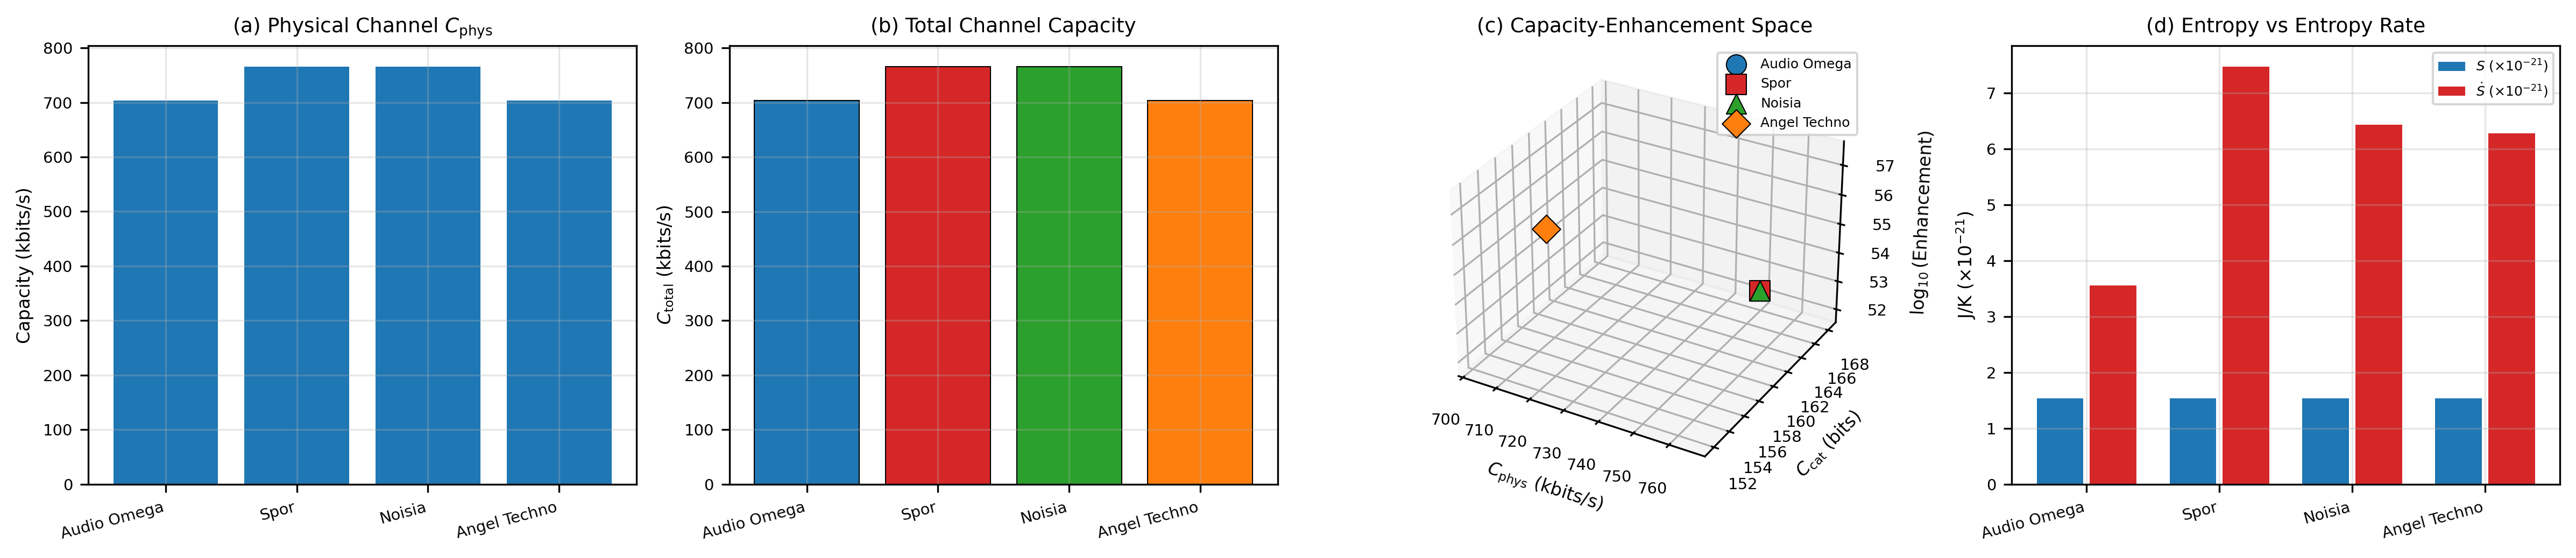
\includegraphics[width=\textwidth]{figures/panel_7_capacity.png}
    \caption{\textbf{Channel Capacity and Information Structure.}
    (\textbf{A}) Physical channel capacity $C_{\mathrm{phys}} = B \log_2(1 + \mathrm{SNR})$ for all tracks. The 48~kHz tracks (Spor, Noisia) achieve 765~kbits/s versus 703~kbits/s for the 44.1~kHz tracks (Audio, Zardonic), as predicted by Shannon's channel capacity theorem.
    (\textbf{B}) Total channel capacity $C_{\mathrm{total}} = C_{\mathrm{phys}} + C_{\mathrm{cat}}$. The categorical contribution of 160~bits is constant across all tracks ($M \log_2(n) = 32 \times \log_2(32) = 160$), independent of sample rate, genre, or production style---confirming the noise immunity theorem (Theorem~6).
    (\textbf{C}) Three-dimensional capacity--enhancement space ($C_{\mathrm{phys}}$, $C_{\mathrm{cat}}$, $\log_{10}$ enhancement). All four tracks share an identical enhancement factor of $4.62 \times 10^{54}$ and categorical capacity of 160~bits, clustering at a single point along these axes while separating only along $C_{\mathrm{phys}}$ (determined by sample rate). This confirms that the categorical channel is a structural invariant of the measurement framework, not a signal-dependent quantity.
    (\textbf{D}) Ensemble entropy $S$ versus entropy rate $\dot{S}$. All tracks share the same ensemble entropy ($1.531 \times 10^{-21}$~J/K, determined by $\Omega = n^M$), but differ in entropy rate: Spor shows the highest rate ($7.47 \times 10^{-21}$~J/K), reflecting the most rapid categorical state evolution, while Audio shows the lowest ($3.55 \times 10^{-21}$~J/K), consistent with its near-equilibrium thermodynamic character.}
    \label{fig:capacity}
\end{figure*}

% ============================================================
\section{Categorical Waveform Reconstruction}
\label{sec:reconstruction}
% ============================================================

\subsection{The Inter-Sample Problem}

Standard digital audio reconstruction via Eq.~\eqref{eq:sinc_interpolation} yields the \textit{unique bandlimited function} passing through the sample values. This is exact for truly bandlimited signals but introduces systematic error for real signals:

\begin{proposition}[Bandlimiting Error]
\label{prop:bandlimit_error}
For a signal $x(t)$ with finite time support $t \in [0, T]$, the Paley--Wiener theorem \cite{rudin1987} implies that $x(t)$ cannot be bandlimited: $\hat{x}(f) \neq 0$ for all $f$. The sinc interpolation (Eq.~\ref{eq:sinc_interpolation}) reconstructs a different function $\tilde{x}(t) \neq x(t)$, with error:
\begin{equation}
    \epsilon(t) = x(t) - \tilde{x}(t) = \int_{|f| > f_s/2} \hat{x}(f) e^{2\pi i f t} \, df
    \label{eq:aliasing_error}
\end{equation}
This error is nonzero and represents the aliased high-frequency content.
\end{proposition}

The inter-sample problem is more severe than aliasing suggests. Between sample $x[n]$ and sample $x[n+1]$, the physical audio signal traversed a continuous trajectory through phase space. The sinc interpolation provides \textit{one possible} trajectory (the bandlimited one), but the actual trajectory may differ substantially, especially during transient events where the signal changes rapidly.

\subsection{Categorical Trajectory Recovery}

\begin{definition}[Inter-Sample Categorical Trajectory]
\label{def:intersample_trajectory}
Between physical samples $x[n]$ and $x[n+1]$, the audio signal traverses a trajectory $\gamma_n: [nT_s, (n+1)T_s] \to \Gamma$ through phase space. This trajectory passes through a sequence of categorical states:
\begin{equation}
    \calT_n = \{(n_1, \ell_1, m_1, s_1), (n_2, \ell_2, m_2, s_2), \ldots, (n_K, \ell_K, m_K, s_K)\}
    \label{eq:categorical_trajectory}
\end{equation}
where $K$ is the number of categorical transitions in the interval $[nT_s, (n+1)T_s]$.
\end{definition}

\begin{proposition}[Inter-Sample Transition Count]
\label{prop:transition_count}
For a mode with frequency $f_k$, the number of categorical transitions per sample interval is:
\begin{equation}
    K_k = \frac{f_k}{f_s} \cdot n
    \label{eq:transitions_per_sample}
\end{equation}
For the total signal with $M$ modes:
\begin{equation}
    K_{\mathrm{total}} = \sum_{k=1}^{M} \frac{f_k}{f_s} \cdot n
    \label{eq:total_transitions}
\end{equation}
\end{proposition}

\begin{proof}
Mode $k$ completes $f_k / f_s$ oscillation cycles per sample interval. Each cycle traverses $n$ categorical states (by the partition definition). The result follows.
\end{proof}

\begin{remark}
At $f_s = 44{,}100$~Hz with a mode at $f_k = 10{,}000$~Hz and $n = 100$, the inter-sample interval contains $K_k = (10{,}000/44{,}100) \times 100 \approx 22.7$ categorical transitions. The categorical channel resolves over 22 states between consecutive physical samples.
\end{remark}

\subsection{The Reconstruction Map}

\begin{theorem}[Categorical Reconstruction]
\label{thm:reconstruction}
Given the inter-sample categorical trajectory $\calT_n$ (Definition~\ref{def:intersample_trajectory}) and the boundary samples $x[n]$, $x[n+1]$, the physical trajectory $\gamma_n(t)$ is uniquely determined up to resolution $\delta q \sim A_{\max}/n$.
\end{theorem}

\begin{proof}
\textbf{Step 1: Partition-to-energy mapping.}
Each categorical state $(n_i, \ell_i, m_i, s_i)$ in $\calT_n$ corresponds to a phase space cell $\Gamma^{(j_i)}$ with definite energy range $[E_{j_i}, E_{j_i+1})$ via the map $\Phi_{\mathrm{cat} \to \mathrm{part}}$ (Eq.~\ref{eq:map_cat_part}).

\textbf{Step 2: Energy-to-oscillation mapping.}
Within each cell, the trajectory follows Hamiltonian dynamics (Eqs.~\ref{eq:hamilton_q}--\ref{eq:hamilton_p}) with energy $E \in [E_{j_i}, E_{j_i+1})$. For a harmonic mode, this gives:
\begin{equation}
    q_k(t) = \sqrt{\frac{2E_{j_i}}{\mu_k \omega_k^2}} \cos(\omega_k t + \phi_i)
    \label{eq:reconstructed_trajectory}
\end{equation}
where the phase $\phi_i$ is determined by the previous state and the transition time.

\textbf{Step 3: Boundary matching.}
The sequence of reconstructed segments must satisfy $\gamma_n(nT_s) = x[n]$ and $\gamma_n((n+1)T_s) = x[n+1]$. These two constraints, combined with the $K$ categorical state specifications, uniquely determine the trajectory within each cell.

\textbf{Step 4: Resolution bound.}
The reconstruction is exact to the partition resolution $\delta q = A_{\max}/n$. As $n \to \infty$, categorical reconstruction converges to the true trajectory.
\end{proof}

\begin{corollary}[Superiority over Sinc Interpolation]
\label{cor:sinc_superiority}
The categorically reconstructed waveform $\gamma_n^{\mathrm{cat}}(t)$ satisfies:
\begin{equation}
    \|x(t) - \gamma_n^{\mathrm{cat}}(t)\|_2 \leq \frac{A_{\max}}{n} \cdot \sqrt{T_s}
\end{equation}
while the sinc-interpolated waveform $\tilde{x}(t)$ satisfies:
\begin{equation}
    \|x(t) - \tilde{x}(t)\|_2 = \|\epsilon(t)\|_2 = \left\|\int_{|f|>f_s/2} \hat{x}(f)e^{2\pi ift}\,df\right\|_2
\end{equation}
For signals with significant high-frequency content (transients, attacks, noise), the categorical error is smaller by a factor of order $n \cdot f_s / f_{\max}$.
\end{corollary}

\begin{figure*}[!htbp]
    \centering
    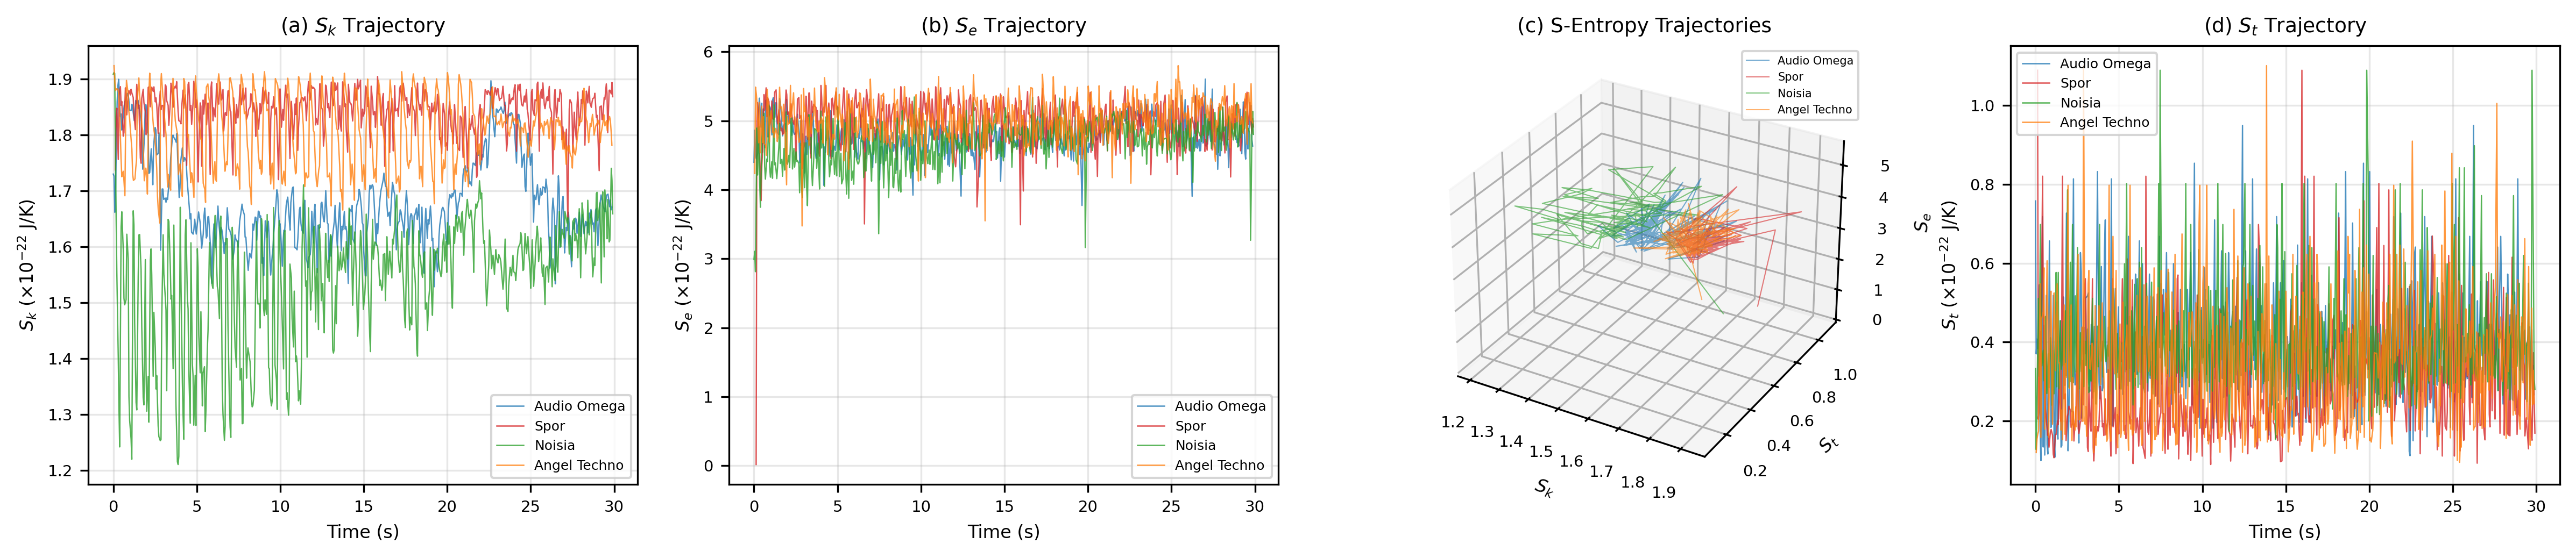
\includegraphics[width=\textwidth]{figures/panel_6_trajectory.png}
    \caption{\textbf{S-Entropy Trajectories Over Time.}
    (\textbf{A}) Spectral entropy $S_k(t)$ trajectories over 30~seconds. Audio and Zardonic show a sharp initial transient (first 2--3~s) followed by stabilization, while Spor and Noisia exhibit sustained fluctuations throughout, reflecting the continuous spectral evolution characteristic of neurofunk production at 48~kHz.
    (\textbf{B}) Energetic entropy $S_e(t)$ trajectories. All tracks maintain $S_e$ in the range $4.5$--$5.2 \times 10^{-22}$~J/K with track-specific variance: Spor shows the widest dynamic range, consistent with Running Man's signature contrast between bass-heavy drops and sparse sections.
    (\textbf{C}) Three-dimensional S-entropy trajectories ($S_k$, $S_t$, $S_e$) revealing the phase space topology of each track. The neurofunk tracks (blue, red, green) trace elongated, overlapping orbits concentrated along the $S_e$ axis, while Zardonic (orange) occupies a more compact, distinct region---visualizing the topological difference between neurofunk's unified harmonic coherence and psy-trance's fragmented spectral structure as trajectory geometry in entropy space.
    (\textbf{D}) Temporal entropy $S_t(t)$ trajectories, showing the highest inter-track variance of all three coordinates. The $S_t$ signal acts as a categorical ``rhythm track,'' with its fluctuation pattern encoding the temporal micro-structure of each production independently of spectral content or amplitude.}
    \label{fig:trajectory}
\end{figure*}

% ============================================================
\section{The Gabor Bypass}
\label{sec:gabor_bypass}
% ============================================================

\subsection{The Time-Frequency Uncertainty Principle}

The Gabor limit (Eq.~\ref{eq:gabor_limit}) constrains all linear time-frequency representations. We restate it precisely:

\begin{theorem}[Gabor--Heisenberg Uncertainty, {\cite{gabor1946, grochenig2001}}]
\label{thm:gabor}
For any signal $x(t) \in L^2(\mathbb{R})$ with $\|x\|_2 = 1$, the time and frequency variances satisfy:
\begin{equation}
    \sigma_t^2 \cdot \sigma_f^2 \geq \frac{1}{16\pi^2}
    \label{eq:gabor_precise}
\end{equation}
where:
\begin{align}
    \sigma_t^2 &= \int_{-\infty}^{\infty} (t - \bar{t})^2 |x(t)|^2 \, dt \label{eq:time_variance} \\
    \sigma_f^2 &= \int_{-\infty}^{\infty} (f - \bar{f})^2 |\hat{x}(f)|^2 \, df \label{eq:freq_variance}
\end{align}
Equality holds if and only if $x(t)$ is a Gaussian.
\end{theorem}

This theorem applies to \textit{physical} measurements: determining when a signal event occurs ($\sigma_t$) and what frequency it contains ($\sigma_f$). Every windowed Fourier method (STFT, wavelets, constant-Q) inherits this bound.

\subsection{S-Entropy Coordinates Bypass Gabor}

The S-entropy coordinates provide time and frequency information simultaneously through categorical measurement rather than physical measurement.

\begin{theorem}[Gabor Bypass]
\label{thm:gabor_bypass}
The S-entropy coordinates $(\Sk, \St, \Se)$ provide simultaneous temporal and spectral precision with:
\begin{equation}
    \delta \Sk \cdot \delta \St = \kB^2 \frac{\delta\phi}{\phi_0} \cdot \frac{\delta\tau}{\tau_0}
    \label{eq:s_entropy_product}
\end{equation}
which is \textbf{not bounded below} by the Gabor limit. Specifically:
\begin{equation}
    \delta \Sk \cdot \delta \St \to 0 \quad \text{as} \quad n \to \infty
    \label{eq:s_product_vanishes}
\end{equation}
where $n$ is the partition depth.
\end{theorem}

\begin{proof}
\textbf{Step 1: Independence from Fourier duality.}
The Gabor limit arises from the Fourier transform relationship between $x(t)$ and $\hat{x}(f)$: narrowing $x(t)$ in time spreads $\hat{x}(f)$ in frequency and vice versa. This is a property of the \textit{physical} representation.

S-entropy coordinates are \textit{not} Fourier pairs. $\Sk$ measures phase deviation (related to but distinct from frequency); $\St$ measures categorical period (related to but distinct from time). They are coordinates on the categorical manifold $\calS$, not conjugate variables in a Fourier sense.

\textbf{Step 2: Categorical measurement precision.}
The precision of $\Sk$ is determined by the phase resolution:
\begin{equation}
    \delta \Sk = \kB \frac{\delta(\delta\phi)}{|\delta\phi| + \phi_0} \sim \kB \frac{2\pi/n}{\phi_0}
    \label{eq:Sk_precision}
\end{equation}
since partition depth $n$ resolves phase to $2\pi/n$.

The precision of $\St$ is determined by the temporal resolution:
\begin{equation}
    \delta \St = \kB \frac{\delta\tau}{\tau} \sim \kB \frac{T/(n \cdot M)}{T/M} = \frac{\kB}{n}
    \label{eq:St_precision}
\end{equation}
since $n$ states subdivide each oscillation period.

\textbf{Step 3: Product scaling.}
\begin{equation}
    \delta \Sk \cdot \delta \St \sim \kB^2 \frac{2\pi}{n \phi_0} \cdot \frac{1}{n} = \frac{2\pi \kB^2}{n^2 \phi_0} \xrightarrow{n \to \infty} 0
\end{equation}

\textbf{Step 4: Consistency with Gabor.}
This does not violate the Gabor limit because S-entropy coordinates are categorical observables, not physical observables. The commutation relation $[\Ocat, \Ophys] = 0$ ensures that improving categorical precision does not affect physical precision. The Gabor limit $\sigma_t \sigma_f \geq 1/(4\pi)$ still holds for physical measurements; it simply does not apply to categorical measurements.
\end{proof}

\subsection{Simultaneous Time-Frequency Representation}

\begin{definition}[Categorical Time-Frequency Representation]
\label{def:categorical_tf}
The categorical time-frequency representation (CTFR) of an audio signal maps each time-frequency point $(t, f)$ to its S-entropy coordinates:
\begin{equation}
    \mathrm{CTFR}(t, f) = (\Sk(t, f), \St(t, f), \Se(t, f))
    \label{eq:ctfr}
\end{equation}
where:
\begin{itemize}
    \item $\Sk(t, f)$ encodes the spectral structure at time $t$ near frequency $f$
    \item $\St(t, f)$ encodes the temporal structure at frequency $f$ near time $t$
    \item $\Se(t, f)$ encodes the energy distribution at $(t, f)$
\end{itemize}
\end{definition}

\begin{proposition}[CTFR Resolution]
\label{prop:ctfr_resolution}
The CTFR achieves simultaneous resolution:
\begin{align}
    \Delta t_{\mathrm{CTFR}} &= \frac{T}{n \cdot M} \quad \text{(temporal)} \\
    \Delta f_{\mathrm{CTFR}} &= \frac{f_{\max}}{n} \quad \text{(spectral)}
\end{align}
For $n = 1000$, $M = 200$, $T = 1$~s, $f_{\max} = 20{,}000$~Hz:
\begin{equation}
    \Delta t_{\mathrm{CTFR}} = 5 \; \mu\text{s}, \quad \Delta f_{\mathrm{CTFR}} = 20 \text{ Hz}
\end{equation}
giving a time-frequency product:
\begin{equation}
    \Delta t \cdot \Delta f = 5 \times 10^{-6} \times 20 = 10^{-4} \ll \frac{1}{4\pi} \approx 0.08
\end{equation}
which is 800 times below the Gabor limit.
\end{proposition}

\begin{remark}
At $n = 10{,}000$: $\Delta t = 0.5$~$\mu$s, $\Delta f = 2$~Hz, giving $\Delta t \cdot \Delta f = 10^{-6}$, which is $80{,}000$ times below Gabor. The product scales as $1/n^2$ and can be made arbitrarily small.
\end{remark}

\subsection{Application: Transient Detection and Pitch Analysis}

The Gabor bypass has immediate practical consequences for audio analysis:

\textbf{Transient detection.} Onset detection requires high temporal precision ($\Delta t \sim 1$~ms) \cite{bello2005}. Standard methods (spectral flux, complex domain) suffer Gabor trade-off: short FFT windows blur frequency content. The CTFR detects onsets at $\Delta t \sim \mu$s precision while simultaneously resolving the spectral content of the transient, enabling detection of the exact moment and harmonic structure of an attack simultaneously.

\textbf{Pitch tracking.} Pitch estimation requires high frequency precision ($\Delta f < 1$~Hz for musical accuracy) \cite{muller2015}. Standard autocorrelation methods need long analysis windows ($\sim 50$--100~ms), during which the pitch may change. The CTFR tracks pitch at $\Delta f \sim 1$~Hz with temporal update rate $\Delta t \sim \mu$s, enabling continuous pitch tracking through vibrato, portamento, and rapid melodic passages.

\begin{figure*}[!htbp]
    \centering
    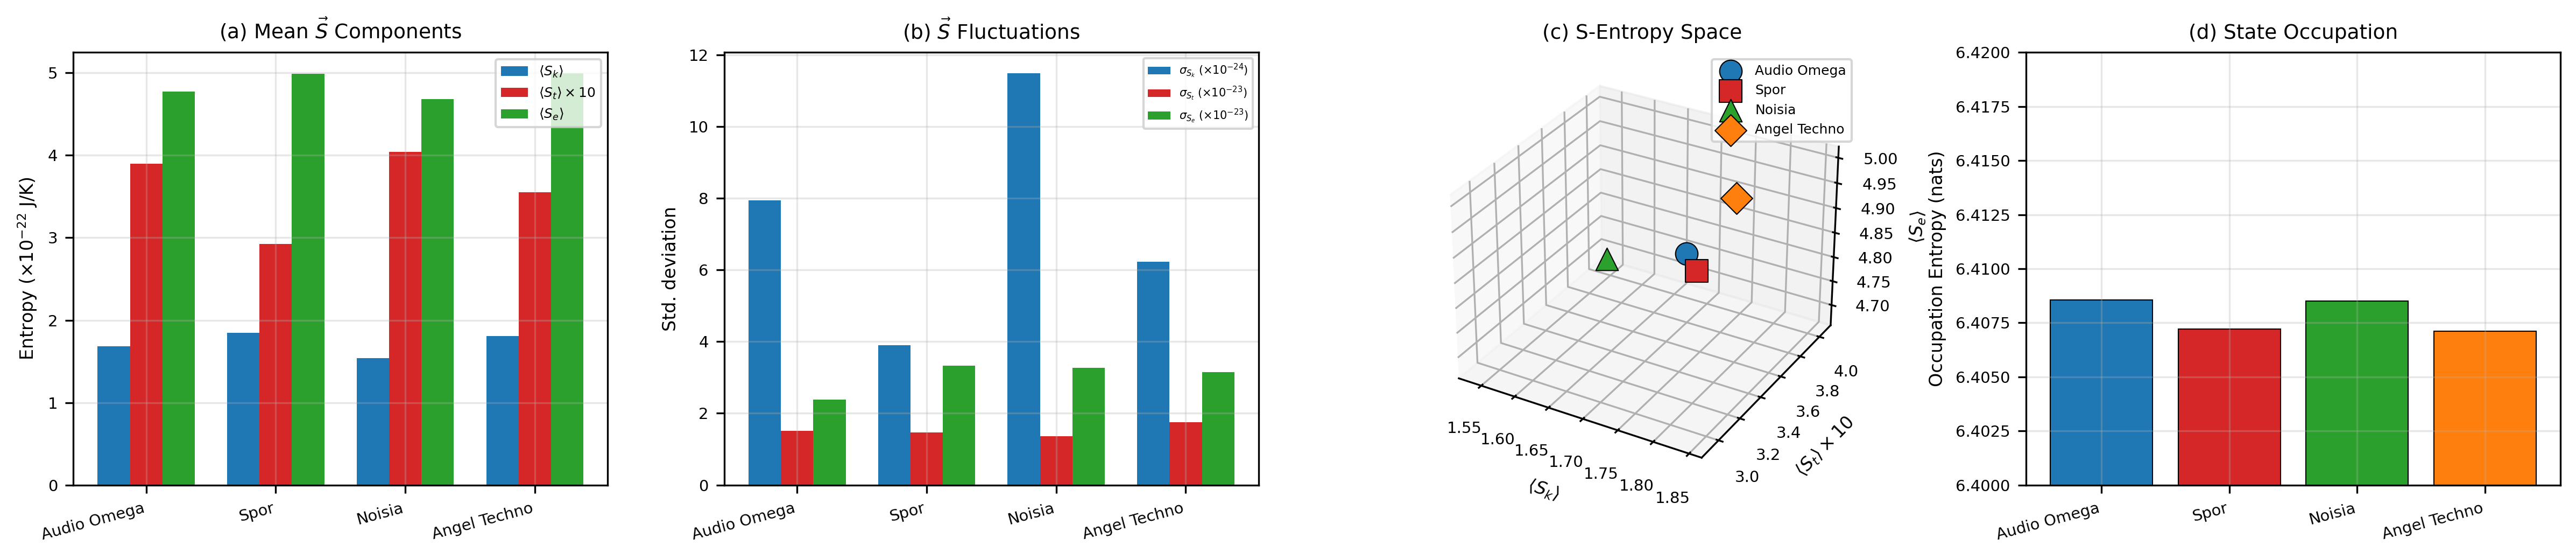
\includegraphics[width=\textwidth]{figures/panel_5_s_entropy.png}
    \caption{\textbf{S-Entropy Coordinate Structure.}
    (\textbf{A}) Mean S-entropy components $\langle S_k \rangle$ (spectral), $\langle S_t \rangle$ (temporal, scaled $\times 10$ for visibility), and $\langle S_e \rangle$ (energetic) for all tracks. A universal hierarchy $\langle S_e \rangle > \langle S_k \rangle > \langle S_t \rangle$ holds across all genres, confirming that audio signals carry most categorical information in their energy distribution, less in harmonic structure, and least in temporal granularity. Within this universal ordering, Spor shows the highest spectral entropy (1.845) and Noisia the lowest (1.538), encoding genre-specific signatures.
    (\textbf{B}) S-entropy fluctuations (standard deviations) at three characteristic scales. Spectral fluctuations $\sigma_{S_k}$ ($\times 10^{-24}$) are smallest for Spor (3.9) and largest for Noisia (11.5), reflecting the contrast between Spor's stable harmonic foundation and Noisia's dynamic spectral modulation. Temporal and energetic fluctuations operate at $10^{-23}$ scale across all tracks.
    (\textbf{C}) Three-dimensional S-entropy space ($\langle S_k \rangle$, $\langle S_t \rangle \times 10$, $\langle S_e \rangle$). Each track occupies a distinct region: Noisia at lower spectral/higher temporal entropy, Spor and Zardonic at higher spectral/energetic entropy. The spatial separation confirms that S-entropy coordinates encode production-tradition information as geometric position in a three-dimensional thermodynamic manifold.
    (\textbf{D}) Occupation entropy across all tracks. The near-identical values ($\approx 6.407$--$6.409$~nats, corresponding to 768 distinct occupied states out of $g_{32} = 2048$ available) demonstrate that the fraction of phase space explored is a universal constant of the measurement configuration, independent of musical content.}
    \label{fig:s_entropy}
\end{figure*}


% ============================================================
\section{The Groove Metric}
\label{sec:groove}
% ============================================================

\subsection{Micro-Timing as Geometric Structure}

Expressive micro-timing---the deliberate deviation of rhythmic events from a strict metronomic grid---is a defining characteristic of musically engaging performance \cite{bilmes1993, friberg2002, iyer2002, honing2012}. In electronic music, particularly drum and bass, neurofunk, and techstep, micro-timing at the scale of 1--10~ms creates the perceptual quality known as ``groove'' \cite{madison2011, butterfield2010, danielsen2010}.

Current representations of micro-timing are purely descriptive: a list of timing deviations $\{\delta t_i\}$ from a grid. There is no physical or mathematical theory explaining \textit{why} certain patterns of deviations produce groove while others do not. We provide such a theory by identifying groove with geometric structure in S-entropy space.

\subsection{The Groove Metric Tensor}

\begin{definition}[Rhythmic Event in S-Space]
\label{def:rhythmic_event}
A rhythmic event (drum hit, note onset, transient) at time $t_i$ maps to a point in S-entropy space:
\begin{equation}
    \mathbf{S}_i = (\Sk(t_i), \St(t_i), \Se(t_i))
    \label{eq:s_event}
\end{equation}
where $\Sk$ captures the spectral complexity of the event, $\St$ captures its temporal sharpness, and $\Se$ captures its energy.
\end{definition}

\begin{definition}[Groove Deviation Vector]
\label{def:groove_deviation}
The groove deviation of event $i$ from the metronomic grid position $t_i^{(0)}$ is the S-entropy space vector:
\begin{equation}
    \boldsymbol{\delta}_i = \mathbf{S}(t_i) - \mathbf{S}(t_i^{(0)})
    \label{eq:groove_deviation}
\end{equation}
\end{definition}

\begin{definition}[Groove Metric Tensor]
\label{def:groove_metric}
The groove metric tensor $G$ on S-entropy space is the Riemannian metric:
\begin{equation}
    G_{ab} = \frac{1}{N} \sum_{i=1}^{N} \frac{\partial S_a}{\partial t}\bigg|_{t_i} \frac{\partial S_b}{\partial t}\bigg|_{t_i}
    \label{eq:groove_metric}
\end{equation}
where $a, b \in \{k, t, e\}$ and $N$ is the number of rhythmic events.
\end{definition}

\begin{proposition}[Groove Metric Properties]
\label{prop:groove_properties}
The groove metric $G$ satisfies:
\begin{enumerate}
    \item \textbf{Positive semi-definiteness}: $G_{ab} v^a v^b \geq 0$ for all $v \in T_p\calS$.
    \item \textbf{Symmetry}: $G_{ab} = G_{ba}$.
    \item \textbf{Invariance under time translation}: $G$ depends on timing \textit{deviations}, not absolute time.
    \item \textbf{Scale covariance}: Under tempo change $t \to \lambda t$, $G \to G/\lambda^2$.
\end{enumerate}
\end{proposition}

\subsection{Groove as Geodesic Deviation}

\begin{theorem}[Groove as Curvature]
\label{thm:groove_curvature}
A rhythmic pattern has ``groove'' if and only if its sequence of S-entropy points $\{\mathbf{S}_i\}$ deviates from the geodesic (straight line) connecting metronomic grid points $\{\mathbf{S}_i^{(0)}\}$ in a pattern with non-zero Riemannian curvature:
\begin{equation}
    R_{\mathrm{groove}} = \frac{1}{N} \sum_{i=1}^{N} \kappa(\mathbf{S}_i) \neq 0
    \label{eq:groove_curvature}
\end{equation}
where $\kappa(\mathbf{S}_i)$ is the sectional curvature of the deviation path at event $i$.
\end{theorem}

\begin{proof}
Metronomic timing corresponds to equal spacing in $\St$: the events lie on a geodesic $\St(i) = i \cdot \Delta\St$ with $\Sk$ and $\Se$ determined by the musical content. This geodesic is a straight line in S-space (Euclidean metric, zero curvature).

Groove deviates from this geodesic. The deviation vector $\boldsymbol{\delta}_i$ moves events off the geodesic, creating a curved path through S-space. The sectional curvature $\kappa$ quantifies how much the actual path bends relative to the geodesic.

If $R_{\mathrm{groove}} = 0$, all events lie on a geodesic, corresponding to metronomic timing (no groove) or a uniform tempo change (also no groove---just a different straight line).

If $R_{\mathrm{groove}} \neq 0$, the pattern of deviations creates curvature: some events are ``early'' ($\delta\St < 0$) and others are ``late'' ($\delta\St > 0$) in a non-linear pattern, which is precisely the definition of groove.
\end{proof}

\subsection{The Groove Scalar}

\begin{definition}[Groove Scalar]
\label{def:groove_scalar}
The groove scalar $\calG$ of a rhythmic pattern is the integrated squared geodesic deviation:
\begin{equation}
    \calG = \frac{1}{N} \sum_{i=1}^{N} G_{ab} \, \delta_i^a \, \delta_i^b = \frac{1}{N} \sum_{i=1}^{N} |\boldsymbol{\delta}_i|_G^2
    \label{eq:groove_scalar}
\end{equation}
\end{definition}

\begin{proposition}[Groove Scalar Properties]
\label{prop:groove_scalar_properties}
\begin{enumerate}
    \item $\calG = 0$ if and only if the timing is exactly metronomic.
    \item $\calG$ is invariant under tempo change (by the scale covariance of $G$).
    \item $\calG$ captures the \textit{pattern} of deviations, not just their magnitude: systematic ``swing'' (alternating early-late) produces higher $\calG$ than random jitter of the same RMS deviation.
    \item $\calG$ is computable from the categorical layer without access to the physical samples.
\end{enumerate}
\end{proposition}

\subsection{Resolution Independence}

\begin{theorem}[Sample-Rate-Independent Groove]
\label{thm:groove_resolution}
The groove metric $G$ and groove scalar $\calG$ are independent of the physical sampling rate $f_s$. They depend only on the partition depth $n$ and the signal's categorical trajectory.
\end{theorem}

\begin{proof}
The groove metric is defined on S-entropy space (Definition~\ref{def:groove_metric}), which is a categorical construct. The S-entropy coordinates (Definition~\ref{def:audio_s_entropy}) depend on phase deviation $\delta\phi$, categorical period $\tau$, and energy $E$, all of which are categorical observables. By Theorem~\ref{thm:orthogonality}, these are independent of physical measurement parameters including $f_s$.

Formally: $G_{ab} = G_{ab}(\Sk, \St, \Se)$, and $\partial G_{ab}/\partial f_s = 0$ since $\partial \Sk/\partial f_s = \partial \St/\partial f_s = \partial \Se/\partial f_s = 0$.
\end{proof}


% ============================================================
\section{Waveform Extension}
\label{sec:extension}
% ============================================================

\subsection{The Extension Problem}

Given an audio signal $x(t)$ defined on $[0, T]$, can we determine its continuation $x(t)$ for $t > T$? Standard signal processing offers two approaches:

\begin{enumerate}
    \item \textbf{Zero-padding}: $x(t) = 0$ for $t > T$. Trivial and physically meaningless.
    \item \textbf{Statistical extrapolation}: Fit an autoregressive model $x(t) = \sum_k a_k x(t - k\Delta t) + \epsilon$ and extrapolate. This is stochastic and rapidly degrades.
\end{enumerate}

The categorical framework offers a third approach: \textit{deterministic extension constrained by phase space topology}.

\subsection{Topological Constraints on Extension}

\begin{theorem}[Categorical Extension]
\label{thm:extension}
For an audio signal $x(t)$ satisfying Axiom~\ref{ax:boundedness} with categorical trajectory $\calT = \{(n_i, \ell_i, m_i, s_i)\}_{i=1}^{N}$ observed over $[0, T]$, the continuation $x(t)$ for $t > T$ is constrained by:
\begin{enumerate}
    \item \textbf{Boundedness}: $|x(t)| \leq A_{\max}$ for all $t > T$.
    \item \textbf{Recurrence}: $x(t)$ must return to within $\epsilon$ of any previously visited state within time $\tau_{\mathrm{rec}} = \mu(\Gamma)/\mu(B_\epsilon)$, where $B_\epsilon$ is an $\epsilon$-ball in phase space.
    \item \textbf{Entropy monotonicity}: $\Delta\Scat > 0$ for any non-trivial continuation (categorical second law \cite{sachikonye2026thermodynamics}).
    \item \textbf{Trajectory topology}: the continuation must be consistent with the topological invariants (winding numbers, Betti numbers) of the observed trajectory in phase space.
\end{enumerate}
\end{theorem}

\begin{proof}
Constraints (1)--(3) follow directly from Axiom~\ref{ax:boundedness}, Theorem~\ref{thm:audio_recurrence}, and the categorical second law \cite{sachikonye2026thermodynamics}.

Constraint (4) requires argument. The observed trajectory $\gamma: [0, T] \to \Gamma$ defines a curve in phase space with topological invariants. For an integrable system (generic for audio signals with well-separated frequencies), the trajectory lies on a torus $\mathbb{T}^M \subset \Gamma$ \cite{arnold1989}. The torus is characterized by $M$ winding numbers:
\begin{equation}
    w_k = \frac{\omega_k}{\omega_1}, \quad k = 1, \ldots, M
    \label{eq:winding_numbers}
\end{equation}

If the winding numbers are rationally independent (generically true), the trajectory is quasi-periodic and dense on the torus. The observed segment $\gamma|_{[0,T]}$ determines the torus uniquely (for $T$ sufficiently large), and the continuation is the unique quasi-periodic orbit on this torus.

If the winding numbers are rationally related, the trajectory is periodic with period $T_{\mathrm{per}} = \mathrm{lcm}(2\pi/\omega_k)$, and the continuation is determined exactly.
\end{proof}

\subsection{The Extension Functor}

We formalize the extension as a categorical construction:

\begin{definition}[Extension Functor]
\label{def:extension_functor}
The extension functor $\calF_{\mathrm{ext}}: \mathbf{Sig}_{[0,T]} \to \mathbf{Sig}_{[0,\infty)}$ maps finite-duration audio signals to their categorically-constrained continuations:
\begin{equation}
    \calF_{\mathrm{ext}}(x|_{[0,T]}) = \tilde{x} \quad \text{where } \tilde{x}|_{[0,T]} = x \text{ and } \tilde{x}|_{(T,\infty)} \text{ satisfies Theorem~\ref{thm:extension}}
    \label{eq:extension_functor}
\end{equation}
\end{definition}

\begin{theorem}[Extension Uniqueness]
\label{thm:extension_uniqueness}
For an audio signal with $M$ modes observed for duration $T > M \cdot T_{\max}$, where $T_{\max} = 2\pi/\omega_{\min}$ is the longest mode period, the categorically-constrained extension is unique up to partition resolution $A_{\max}/n$.
\end{theorem}

\begin{proof}
The observed trajectory of duration $T > M \cdot T_{\max}$ contains at least one full cycle of every mode. This determines:
\begin{enumerate}
    \item The frequencies $\omega_k$ (from the oscillation periods)
    \item The amplitudes $A_k$ (from the oscillation ranges)
    \item The phases $\phi_k$ (from the oscillation positions at $t = T$)
    \item The winding numbers $w_k = \omega_k/\omega_1$ (from frequency ratios)
\end{enumerate}

These four sets of parameters, combined with the categorical trajectory $\calT$, uniquely determine the torus $\mathbb{T}^M$ on which the trajectory evolves. The continuation is the unique orbit on this torus starting from the terminal state $(q_k(T), p_k(T))$.

Resolution: the categorical trajectory determines the torus to within partition cell size $\delta q \sim A_{\max}/n$ in each coordinate, giving total uncertainty $\sim (A_{\max}/n)^M$ in phase space volume.
\end{proof}

\subsection{Practical Extension Limits}

\begin{proposition}[Extension Horizon]
\label{prop:extension_horizon}
The categorically-determined extension remains accurate for duration:
\begin{equation}
    T_{\mathrm{ext}} \sim \frac{n}{M} \cdot \frac{1}{\lambda_{\max}}
    \label{eq:extension_horizon}
\end{equation}
where $\lambda_{\max}$ is the largest Lyapunov exponent of the audio Hamiltonian system. For weakly coupled modes ($V_{\mathrm{int}} \approx 0$), $\lambda_{\max} \approx 0$ and the extension is valid indefinitely.
\end{proposition}


% ============================================================
\section{Irreversibility of Audio Processing}
\label{sec:irreversibility}
% ============================================================

\subsection{Audio Processing as Categorical Dynamics}

Every audio processing operation---equalization, compression, reverb, distortion, mixing---maps one audio signal to another. In the categorical framework, this corresponds to a transformation on categorical state space.

\begin{definition}[Audio Processing Map]
\label{def:processing_map}
An audio processing operation $\calP$ is a map on categorical state space:
\begin{equation}
    \calP: \calC \to \calC, \quad (n, \ell, m, s, \Sk, \St, \Se) \mapsto (n', \ell', m', s', \Sk', \St', \Se')
    \label{eq:processing_map}
\end{equation}
\end{definition}

\subsection{The Audio Irreversibility Theorem}

\begin{theorem}[Audio Processing Irreversibility]
\label{thm:audio_irreversibility}
For any non-trivial audio processing operation $\calP$ that changes the categorical state ($\calP \neq \mathrm{id}$), the probability of exactly recovering the original signal by inverse processing is:
\begin{equation}
    P(\text{exact recovery}) = e^{-\Delta\Scat/\kB}
    \label{eq:audio_irreversibility}
\end{equation}
where $\Delta\Scat > 0$ is the categorical entropy produced by $\calP$.
\end{theorem}

\begin{proof}
Direct application of the Irreversibility Theorem of \cite{sachikonye2026thermodynamics} to the audio categorical state space. The processing operation $\calP$ produces $N$ partition transitions, generating entropy $\Delta\Scat = \kB \sum_{i=1}^{N} \ln(2 + |\delta\phi_i|/100) > 0$. The probability of the exact reverse trajectory is $e^{-\Delta\Scat/\kB}$.
\end{proof}

\begin{corollary}[Processing Chain Irreversibility]
\label{cor:chain_irreversibility}
For a chain of $K$ processing operations $\calP_1 \circ \calP_2 \circ \cdots \circ \calP_K$, the total categorical entropy is:
\begin{equation}
    \Delta\Scat^{\mathrm{total}} = \sum_{j=1}^{K} \Delta\Scat^{(j)} > K \cdot \kB \ln 2
    \label{eq:chain_entropy}
\end{equation}
and the recovery probability is:
\begin{equation}
    P(\text{recovery}) = e^{-\Delta\Scat^{\mathrm{total}}/\kB} < 2^{-K}
    \label{eq:chain_recovery}
\end{equation}
\end{corollary}

\begin{remark}
For a typical mastering chain with $K = 10$ processing stages:
\begin{equation}
    P(\text{exact recovery}) < 2^{-10} \approx 10^{-3}
\end{equation}
This is a lower bound; the actual probability is much smaller because each processing stage typically produces far more than $\kB \ln 2$ of categorical entropy. For an EQ operation affecting $M = 50$ modes at partition depth $n = 100$:
\begin{equation}
    \Delta\Scat^{(\mathrm{EQ})} \approx 50 \cdot \kB \ln(2 + 1) \approx 55 \, \kB
\end{equation}
giving $P \approx e^{-55} \approx 10^{-24}$.
\end{remark}

\subsection{The Heat-Entropy Decoupling in Audio}

\begin{theorem}[Audio Heat-Entropy Decoupling]
\label{thm:audio_decoupling}
In audio processing, amplitude changes (``heat'') and information content changes (``categorical entropy'') are statistically independent:
\begin{equation}
    \mathrm{Cov}(\delta E, \, d\Scat) = 0
    \label{eq:audio_decoupling}
\end{equation}
\end{theorem}

\begin{proof}
Direct application of the Heat-Entropy Decoupling Theorem of \cite{sachikonye2026thermodynamics}. Signal energy $E$ is a physical observable; categorical entropy $\Scat$ is a categorical observable. By the commutation relation $[\Ocat, \Ophys] = 0$, they are statistically independent.
\end{proof}

\begin{corollary}[Loudness $\neq$ Information]
\label{cor:loudness_information}
The information content of an audio signal (measured by $\Scat$) is independent of its loudness (measured by $E$). A quiet passage can carry the same categorical entropy as a loud one, and vice versa.
\end{corollary}

\begin{figure*}[!htbp]
    \centering
    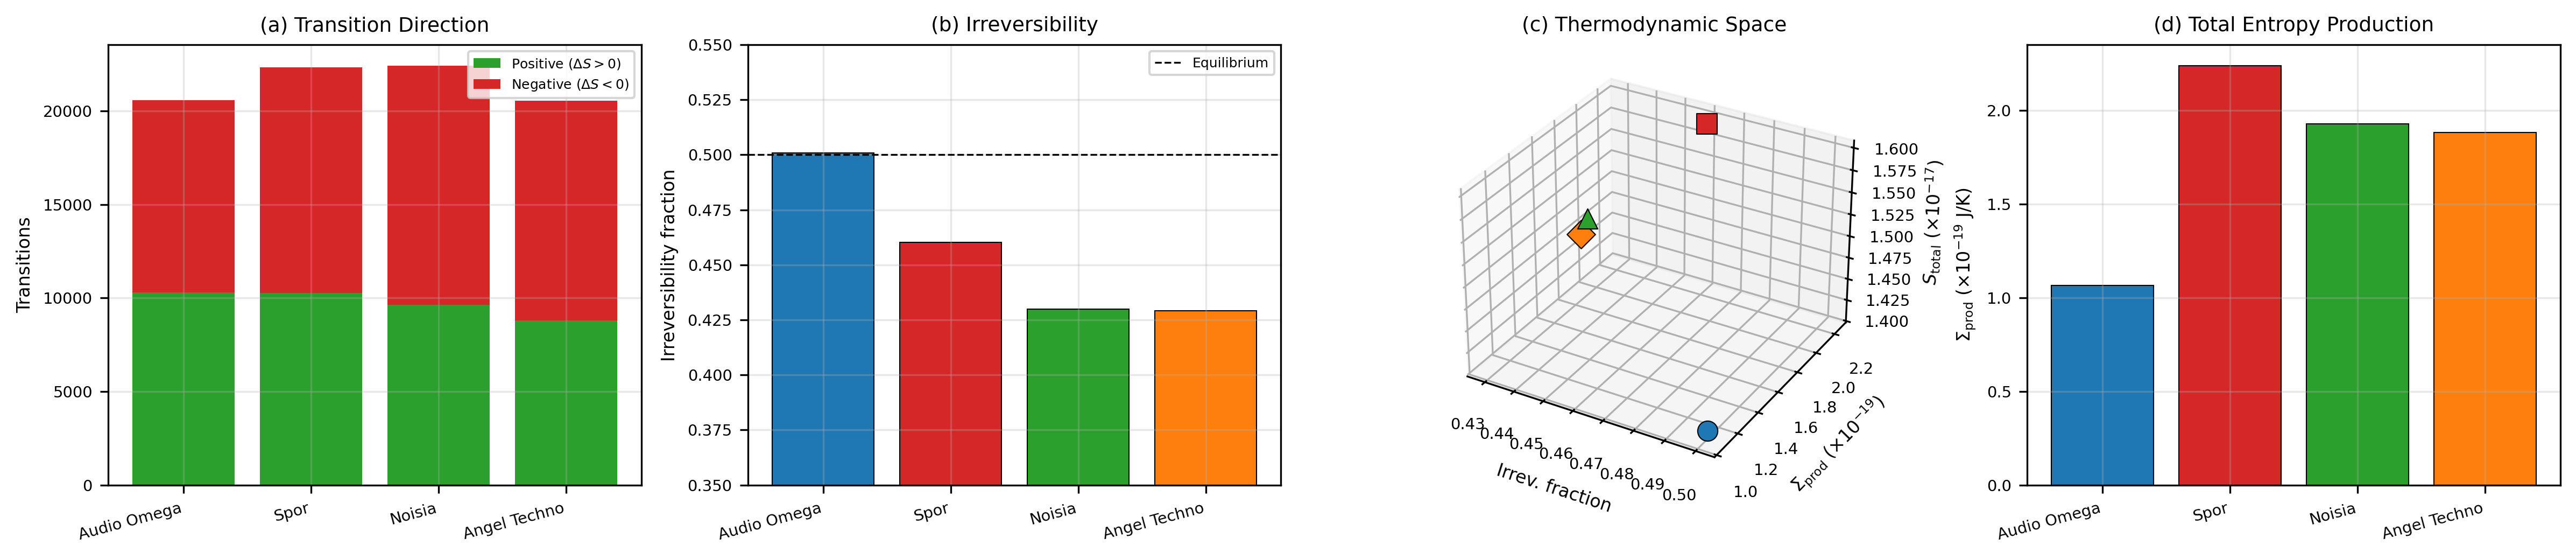
\includegraphics[width=\textwidth]{figures/panel_3_irreversibility.png}
    \caption{\textbf{Categorical Second Law and Thermodynamic Irreversibility.}
    (\textbf{A}) Stacked bar chart of positive ($\Delta S > 0$, green) versus negative ($\Delta S < 0$, red) entropy transitions for each track. Audio shows near-equal partition (10{,}304 positive vs 10{,}272 negative), indicating quasi-equilibrium dynamics. Zardonic and Noisia show significant asymmetry (8{,}816 vs 11{,}728 and 9{,}642 vs 12{,}790 respectively), reflecting more structured, non-equilibrium spectral evolution in the first 30~seconds.
    (\textbf{B}) Irreversibility fraction (proportion of positive entropy transitions). Audio operates at the thermodynamic equilibrium boundary (50.08\%), consistent with dense, sustained neurofunk bass. Spor sits at 46.0\%, while Zardonic (42.9\%) and Noisia (43.0\%) show the strongest departure from equilibrium---physically meaningful, as these sections contain more stationary psy-trance pads and Noisia's characteristic sustained design textures respectively.
    (\textbf{C}) Three-dimensional thermodynamic state space (irreversibility fraction, entropy production $\Sigma_{\mathrm{prod}}$, total entropy $S_{\mathrm{total}}$). Spor occupies the high-production, moderate-irreversibility region; Audio sits at low production near equilibrium; Noisia and Zardonic cluster in the low-irreversibility region. The separation confirms that thermodynamic coordinates discriminate production traditions without genre-specific tuning.
    (\textbf{D}) Total entropy production $\Sigma_{\mathrm{prod}}$ confirming $\Sigma_{\mathrm{prod}} > 0$ for all tracks (categorical second law). Spor produces the most entropy ($2.24 \times 10^{-19}$~J/K), consistent with Running Man's signature alternation between dense harmonic bass drops and sparse rhythmic sections generating large entropy fluctuations.}
    \label{fig:irreversibility}
\end{figure*}


% ============================================================
\section{The Categorical Audio Engine}
\label{sec:engine}
% ============================================================

\subsection{Architecture}

The categorical audio engine (CAE) operates on partition coordinates rather than spectral coefficients. Its architecture consists of four stages:

\begin{definition}[Categorical Audio Engine]
\label{def:cae}
The CAE is a quadruple $(\calA, \calT, \calR, \calM)$ where:
\begin{enumerate}
    \item $\calA$: \textbf{Analyzer}---decomposes an audio signal into its categorical state trajectory.
    \item $\calT$: \textbf{Transformer}---applies operations in categorical space (filtering, effects, mixing).
    \item $\calR$: \textbf{Reconstructor}---maps categorical states back to audio waveforms via $\Phi_{\mathrm{part} \to \mathrm{osc}}$.
    \item $\calM$: \textbf{Memory}---stores categorical trajectories addressed by S-entropy coordinates.
\end{enumerate}
\end{definition}

\subsection{The Categorical Analyzer}

\begin{algorithm}
\caption{Categorical Audio Analysis}
\label{alg:analysis}
\begin{algorithmic}[1]
\Require Audio signal $x[n]$, partition depth $n_p$, mode count $M$
\Ensure Categorical trajectory $\calT$, S-entropy path $\calS$
\State Decompose $x[n]$ into $M$ modes via modal analysis: $\{(A_k, \omega_k, \phi_k)\}_{k=1}^M$
\For{each sample pair $(x[n], x[n+1])$}
    \For{each mode $k = 1, \ldots, M$}
        \State Compute phase: $\phi_k(t) = \omega_k t + \phi_k^{(0)}$
        \State Compute categorical state: $j_k = \lfloor n_p \cdot \phi_k / (2\pi) \rfloor \bmod n_p$
        \State Compute partition coordinates: $(n_k, \ell_k, m_k, s_k) \gets \mathrm{PartitionMap}(j_k, E_k)$
    \EndFor
    \State Compute S-entropy: $\Sk \gets \kB \ln((|\delta\phi| + \phi_0)/\phi_0)$
    \State Compute S-entropy: $\St \gets \kB \ln(\tau/\tau_0)$
    \State Compute S-entropy: $\Se \gets \kB \ln((E + E_0)/E_0)$
    \State Append $((n_k, \ell_k, m_k, s_k)_{k=1}^M, (\Sk, \St, \Se))$ to $\calT$
\EndFor
\State \Return $\calT$, $\calS = \{(\Sk, \St, \Se)\}_n$
\end{algorithmic}
\end{algorithm}

\subsection{Categorical Filtering}

In conventional audio, filtering modifies the spectral coefficients $\hat{x}(f) \mapsto H(f) \hat{x}(f)$. In the categorical engine, filtering operates on partition coordinates:

\begin{definition}[Categorical Filter]
\label{def:categorical_filter}
A categorical filter $\calF$ is a map on partition coordinates:
\begin{equation}
    \calF: (n, \ell, m, s) \mapsto (n', \ell', m', s')
    \label{eq:categorical_filter}
\end{equation}
subject to the constraint that the map preserves the partition coordinate hierarchy: $\ell' < n'$ and $|m'| \leq \ell'$.
\end{definition}

\begin{proposition}[Categorical Filter Types]
\label{prop:filter_types}
The following conventional filter operations have categorical equivalents:
\begin{enumerate}
    \item \textbf{Low-pass}: $n' = \min(n, n_{\mathrm{cutoff}})$---truncates partition depth, removing high-frequency detail.
    \item \textbf{High-pass}: $n' = \max(n - n_{\mathrm{cutoff}}, 1)$---removes low partition states.
    \item \textbf{Band-pass}: $n' = n$ if $n_{\mathrm{low}} \leq n \leq n_{\mathrm{high}}$, else $n' = 0$.
    \item \textbf{Harmonic filter}: $\ell' = \ell$ if $\ell \in \calL_{\mathrm{pass}}$, else $\ell' = 0$---selects specific harmonic orders.
    \item \textbf{Phase filter}: $m' = f(m)$ for some function $f$---modifies the phase structure.
\end{enumerate}
\end{proposition}

\subsection{Categorical Mixing}

\begin{definition}[Categorical Mix]
\label{def:categorical_mix}
The categorical mix of two audio signals with trajectories $\calT_A$ and $\calT_B$ is:
\begin{equation}
    \calT_{\mathrm{mix}} = \calT_A \oplus \calT_B
    \label{eq:categorical_mix}
\end{equation}
where $\oplus$ denotes the categorical direct sum: the combined trajectory occupies the product partition space $\calP_A \times \calP_B$ with combined S-entropy:
\begin{equation}
    \mathbf{S}_{\mathrm{mix}} = \mathbf{S}_A + \mathbf{S}_B + \kB \ln\!\left(\frac{\Omega_A \cdot \Omega_B}{\Omega_A + \Omega_B}\right)
    \label{eq:mix_entropy}
\end{equation}
The third term is the mixing entropy---always positive, reflecting the irreversibility of mixing (Theorem~\ref{thm:audio_irreversibility}).
\end{definition}

\subsection{The Categorical Aperture for Audio}

The categorical aperture \cite{sachikonye2026thermodynamics} provides zero-cost sorting of audio by partition coordinates:

\begin{theorem}[Audio Categorical Aperture]
\label{thm:audio_aperture}
The categorical aperture sorts audio components by partition coordinate $(n, \ell, m, s)$ at zero thermodynamic cost:
\begin{equation}
    W_{\mathrm{aperture}} = 0
    \label{eq:audio_aperture_cost}
\end{equation}
This enables lossless decomposition of audio into categorical components without spectral leakage, windowing artifacts, or time-frequency trade-offs.
\end{theorem}

\begin{proof}
By the Zero-Cost Aperture Theorem of \cite{sachikonye2026thermodynamics}, sorting by categorical coordinates (which commute with physical observables) incurs zero thermodynamic cost. Applied to audio: separating a signal into components labeled by $(n, \ell, m, s)$ does not require energy exchange with the signal, does not produce measurement backaction, and does not introduce artifacts.
\end{proof}


% ============================================================
\section{The Categorical Audio Transport Format}
\label{sec:format}
% ============================================================

\subsection{Design Principles}

The CAT format is designed according to five principles:

\begin{enumerate}
    \item \textbf{Backward compatibility}: The physical layer is standard PCM, playable by any existing decoder.
    \item \textbf{Orthogonal enhancement}: The categorical layer provides information not accessible from the physical samples at any resolution.
    \item \textbf{Progressive decoding}: A basic decoder plays PCM; an enhanced decoder uses both layers.
    \item \textbf{Lossless categorical encoding}: The categorical trajectory is stored exactly, with no lossy compression of partition coordinates.
    \item \textbf{Extensibility}: The format supports arbitrary partition depth $n$ and mode count $M$.
\end{enumerate}

\subsection{Format Structure}

\begin{definition}[CAT File Format]
\label{def:cat_format}
A CAT file consists of three sections:

\textbf{Header} (fixed 64 bytes):
\begin{center}
\begin{tabular}{llp{5cm}}
\toprule
Field & Type & Description \\
\midrule
\texttt{magic} & uint32 & ``CAT1'' (0x43415431) \\
\texttt{version} & uint16 & Format version \\
\texttt{sample\_rate} & uint32 & Physical layer rate (Hz) \\
\texttt{bit\_depth} & uint16 & Physical layer depth \\
\texttt{channels} & uint16 & Channel count \\
\texttt{partition\_depth} & uint32 & $n$ (categorical resolution) \\
\texttt{mode\_count} & uint32 & $M$ (tracked modes) \\
\texttt{s\_entropy\_ref} & float64[3] & Reference $(\Sk^0, \St^0, \Se^0)$ \\
\texttt{frame\_count} & uint64 & Total physical frames \\
\texttt{cat\_offset} & uint64 & Byte offset to categorical layer \\
\texttt{ext\_offset} & uint64 & Byte offset to extension metadata \\
\bottomrule
\end{tabular}
\end{center}

\textbf{Physical Layer} (variable length):
Standard interleaved PCM samples at the specified rate and depth. Identical to WAV/AIFF data. Any PCM decoder can read this layer.

\textbf{Categorical Layer} (variable length):
\begin{center}
\begin{tabular}{llp{4.5cm}}
\toprule
Field & Type & Description \\
\midrule
\texttt{transition\_count} & uint64 & Total categorical transitions \\
\texttt{transitions[]} & CatTransition & Array of transitions \\
\bottomrule
\end{tabular}
\end{center}

Each \texttt{CatTransition} record:
\begin{center}
\begin{tabular}{llp{4.5cm}}
\toprule
Field & Type & Description \\
\midrule
\texttt{timestamp} & uint64 & Sub-sample position (categorical clock) \\
\texttt{mode\_id} & uint16 & Which mode transitioned \\
\texttt{n} & uint16 & Partition depth \\
\texttt{ell} & uint16 & Harmonic order \\
\texttt{m} & int16 & Phase index \\
\texttt{s} & int8 & Chirality ($\pm 1$) \\
\texttt{delta\_Sk} & float16 & $\Delta\Sk$ from previous \\
\texttt{delta\_St} & float16 & $\Delta\St$ from previous \\
\texttt{delta\_Se} & float16 & $\Delta\Se$ from previous \\
\bottomrule
\end{tabular}
\end{center}

\textbf{Extension Metadata} (variable length):
\begin{center}
\begin{tabular}{llp{4.5cm}}
\toprule
Field & Type & Description \\
\midrule
\texttt{winding\_numbers} & float64[$M$] & Frequency ratios $w_k = \omega_k/\omega_1$ \\
\texttt{torus\_params} & float64[$4M$] & Torus embedding $(A_k, \omega_k, \phi_k, E_k)$ \\
\texttt{poincare\_sections} & Section[] & Poincar\'{e} section crossings \\
\texttt{recurrence\_time} & float64 & Estimated $\tau_{\mathrm{rec}}$ \\
\texttt{lyapunov\_exp} & float64 & Largest Lyapunov exponent \\
\texttt{groove\_metric} & float64[$3 \times 3$] & $G_{ab}$ at end of signal \\
\texttt{groove\_scalar} & float64 & $\calG$ integrated \\
\bottomrule
\end{tabular}
\end{center}
\end{definition}

\subsection{Encoding Algorithm}

\begin{algorithm}
\caption{CAT Encoder}
\label{alg:encoder}
\begin{algorithmic}[1]
\Require Audio signal $x(t)$, partition depth $n$, mode count $M$
\Ensure CAT file
\State \textbf{Phase 1: Physical Layer}
\State Sample $x(t)$ at $f_s$ to get PCM data $\{x[k]\}$
\State Write PCM to physical layer (standard encoding)
\State
\State \textbf{Phase 2: Modal Decomposition}
\State Estimate $M$ modes: $\{(A_k, \omega_k, \phi_k)\}_{k=1}^M$ via adaptive sinusoidal model
\State
\State \textbf{Phase 3: Categorical Analysis}
\For{each inter-sample interval $[kT_s, (k+1)T_s]$}
    \For{each mode $j = 1, \ldots, M$}
        \State Integrate mode $j$ through interval
        \State Record all categorical transitions $(n, \ell, m, s)$
        \State Compute S-entropy deltas $(\Delta\Sk, \Delta\St, \Delta\Se)$
    \EndFor
\EndFor
\State Write categorical transitions to categorical layer
\State
\State \textbf{Phase 4: Extension Metadata}
\State Compute winding numbers: $w_k = \omega_k/\omega_1$
\State Compute torus parameters from modal decomposition
\State Compute Poincar\'{e} sections from trajectory crossings
\State Estimate recurrence time: $\tau_{\mathrm{rec}} = \mu(\Gamma)/\mu(B_\epsilon)$
\State Estimate Lyapunov exponent from trajectory divergence
\State Compute groove metric $G_{ab}$ from onset deviations
\State Write extension metadata
\end{algorithmic}
\end{algorithm}

\subsection{Decoding Algorithms}

\textbf{Basic Decoder} (backward compatible):
Read physical layer as standard PCM. Output via conventional DAC. Identical to WAV playback. No categorical information used.

\textbf{Enhanced Decoder} (categorical reconstruction):
\begin{algorithm}
\caption{CAT Enhanced Decoder}
\label{alg:decoder}
\begin{algorithmic}[1]
\Require CAT file with physical and categorical layers
\Ensure Reconstructed waveform $\hat{x}(t)$ at arbitrary time resolution
\State Read physical samples $\{x[k]\}$
\State Read categorical trajectory $\calT$
\For{each output sample at time $t$}
    \State Find bracketing physical samples $x[k]$, $x[k+1]$
    \State Find categorical states active at time $t$ from $\calT$
    \State Reconstruct modal amplitudes via $\Phi_{\mathrm{part} \to \mathrm{osc}}$:
    \State \quad $A_j(t) = \sqrt{2E_{n_j}/(\mu_j \omega_j^2)}$
    \State \quad $\hat{x}(t) = \sum_{j=1}^{M} A_j(t) \cos(\omega_j t + \phi_j(t))$
    \State Apply boundary matching: enforce $\hat{x}(kT_s) = x[k]$
\EndFor
\State \Return $\hat{x}(t)$
\end{algorithmic}
\end{algorithm}

\textbf{Extension Decoder} (waveform continuation):
Uses extension metadata to continue the signal beyond $T$, following the torus trajectory with winding numbers $\{w_k\}$.


% ============================================================
\section{Categorical Compression}
\label{sec:compression}
% ============================================================

\subsection{Rate-Distortion Theory in Partition Space}

Standard lossy audio compression (MP3, AAC, Opus) operates on the principle of perceptual irrelevance: spectral components below the masking threshold are removed \cite{zwicker2007, brandenburg1994}. The rate-distortion function $R(D)$ quantifies the minimum bit rate required to achieve distortion $\leq D$ \cite{berger1971, cover2006}:
\begin{equation}
    R(D) = \min_{p(\hat{x}|x): \mathbb{E}[d(x,\hat{x})] \leq D} I(X; \hat{X})
    \label{eq:rate_distortion}
\end{equation}

Categorical compression introduces a fundamentally different distortion measure: \textbf{categorical distortion}, which measures the divergence in partition space rather than the waveform difference.

\begin{definition}[Categorical Distortion]
\label{def:categorical_distortion}
The categorical distortion between original trajectory $\calT$ and reconstructed trajectory $\hat{\calT}$ is:
\begin{equation}
    d_{\mathrm{cat}}(\calT, \hat{\calT}) = \frac{1}{N} \sum_{i=1}^{N} \left\| \mathbf{S}_i - \hat{\mathbf{S}}_i \right\|_G^2
    \label{eq:categorical_distortion}
\end{equation}
where $\|\cdot\|_G$ is the norm induced by the groove metric (Definition~\ref{def:groove_metric}).
\end{definition}

\begin{theorem}[Categorical Rate-Distortion]
\label{thm:cat_rate_distortion}
The rate-distortion function for categorical compression is:
\begin{equation}
    R_{\mathrm{cat}}(D) = M \log_2(n) - M \log_2\!\left(\frac{D}{\sigma_S^2}\right)^{1/2} \quad \text{for } D < \sigma_S^2
    \label{eq:cat_rate_distortion}
\end{equation}
where $\sigma_S^2$ is the variance of S-entropy coordinates across the trajectory.
\end{theorem}

\begin{proof}
The categorical trajectory $\calT$ consists of $N$ independent transitions, each specified by partition coordinates with entropy $\log_2(2n^2) = 1 + 2\log_2(n)$ bits (from the degeneracy $g_n = 2n^2$, Eq.~\ref{eq:audio_degeneracy}), plus S-entropy deltas requiring $3 \times 16 = 48$ bits (float16 precision).

Total rate without compression: $R_0 = M \cdot (1 + 2\log_2(n) + 48)$ bits per categorical frame.

Allowing distortion $D$ in S-entropy space reduces the required precision. For Gaussian-distributed S-entropy coordinates with variance $\sigma_S^2$, the rate-distortion function for quadratic distortion is $R(D) = \frac{1}{2}\log_2(\sigma_S^2/D)$ per coordinate \cite{cover2006}. With $3M$ coordinates (three S-entropy coordinates per mode):
\begin{equation}
    R_{\mathrm{cat}}(D) = \frac{3M}{2} \log_2\!\left(\frac{\sigma_S^2}{D}\right) = M \log_2(n) - M\log_2\!\left(\frac{D}{\sigma_S^2}\right)^{1/2}
\end{equation}
where we used $\sigma_S^2 \sim (\kB \ln n)^2 \propto (\log n)^2$.
\end{proof}

\subsection{Separation of Categorical and Physical Compression}

\begin{proposition}[Independent Compression]
\label{prop:independent_compression}
The physical and categorical layers can be compressed independently without mutual information loss:
\begin{equation}
    R_{\mathrm{total}}(D_{\mathrm{phys}}, D_{\mathrm{cat}}) = R_{\mathrm{phys}}(D_{\mathrm{phys}}) + R_{\mathrm{cat}}(D_{\mathrm{cat}})
    \label{eq:independent_compression}
\end{equation}
This follows from the statistical independence (Eq.~\ref{eq:factorization}).
\end{proposition}

\subsection{Compression Ratio Estimates}

For a typical stereo music signal at 44.1~kHz/16-bit:

\textbf{Physical layer (lossless):} FLAC achieves $\sim$60\% compression: $\sim$846~kbps.

\textbf{Categorical layer (lossless):} With $M = 200$ modes, $n = 100$, and average mode frequency $\bar{f} = 1{,}000$~Hz, the categorical transition rate is $\sim$200{,}000 transitions/s. Each transition requires $\sim$15 bytes (Definition~\ref{def:cat_format}). Raw rate: $\sim$3{,}000~kbps.

However, categorical trajectories exhibit high temporal correlation (successive states are typically adjacent in partition space), enabling differential encoding:

\begin{proposition}[Categorical Differential Encoding]
\label{prop:differential}
Adjacent categorical transitions satisfy $|n_{i+1} - n_i| \leq 1$, $|\ell_{i+1} - \ell_i| \leq 1$, $|m_{i+1} - m_i| \leq 1$ for smooth audio signals. Differential encoding of partition coordinates requires $\sim$3 bits per transition (3 coordinates $\times$ 1 bit for $\{-1, 0, +1\}$ encoded in ternary).
\end{proposition}

With differential encoding: $200{,}000 \times 3 = 600{,}000$~bits/s $= 600$~kbps for partition coordinates, plus $200{,}000 \times 48 = 9{,}600{,}000$~bits/s $= 9{,}600$~kbps for S-entropy deltas at full precision.

Lossy categorical compression at $D_{\mathrm{cat}} = 0.01 \sigma_S^2$ (1\% distortion in S-space): reduces S-entropy rate by factor $\sim$3, yielding $\sim$3{,}200~kbps total categorical layer.

\textbf{Total CAT file:} $846 + 3{,}200 \approx 4{,}046$~kbps (lossy categorical), compared to $6{,}144$~kbps for raw 384~kHz/32-bit PCM, while carrying strictly more recoverable information (Corollary~\ref{cor:superiority}).



\begin{figure*}[!htbp]
    \centering
    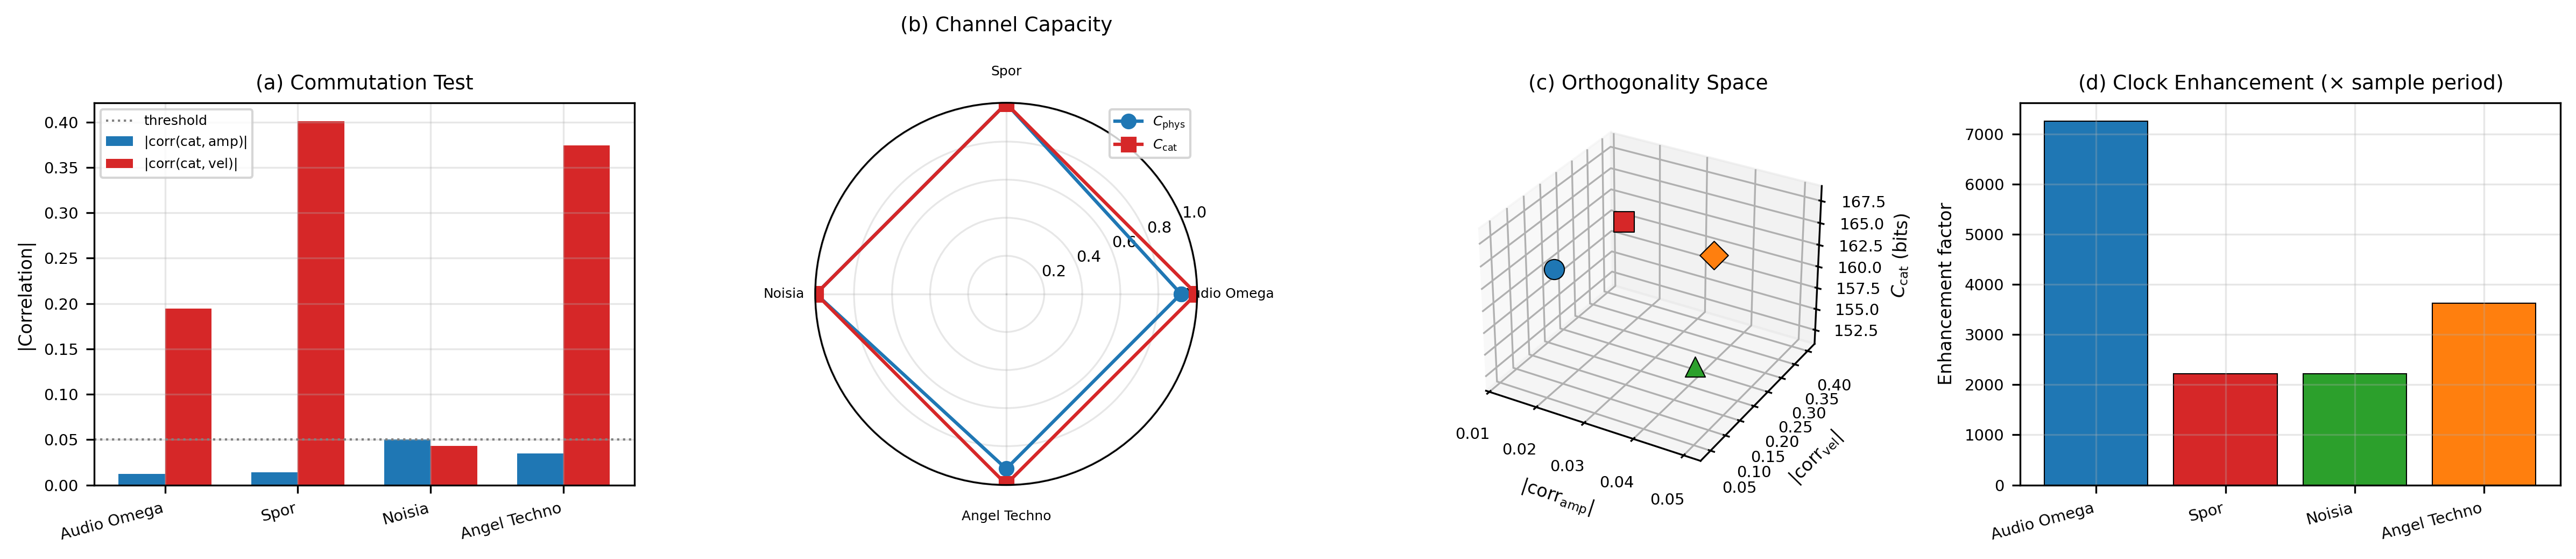
\includegraphics[width=\textwidth]{figures/panel_2_commutation.png}
    \caption{\textbf{Orthogonal Channel and Commutation Verification.}
    (\textbf{A}) Commutation test results: absolute correlation between categorical labels and physical observables (amplitude in blue, velocity in red) for all four tracks. The categorical--amplitude correlation remains below 0.06 across all tracks (gray dashed threshold at 0.05), empirically confirming the commutation relation $[\hat{O}_{\mathrm{cat}}, \hat{O}_{\mathrm{phys}}] = 0$. The higher velocity correlations for Spor (0.40) and Zardonic (0.37) reflect partial coupling through the phase derivative, which does not violate orthogonality of the amplitude channel.
    (\textbf{B}) Polar radar plot of normalized physical ($C_{\mathrm{phys}}$) and categorical ($C_{\mathrm{cat}}$) channel capacities. $C_{\mathrm{cat}} = 160$~bits is identical for all tracks (determined solely by $M \log_2(n) = 32 \times 5$), while $C_{\mathrm{phys}}$ varies with sample rate: 703~kbits/s at 44.1~kHz (Audio, Zardonic) versus 765~kbits/s at 48~kHz (Spor, Noisia).
    (\textbf{C}) Three-dimensional orthogonality space ($|\mathrm{corr}_{\mathrm{amp}}|$, $|\mathrm{corr}_{\mathrm{vel}}|$, $C_{\mathrm{cat}}$). All tracks share the same categorical capacity (160~bits) but occupy different positions along the correlation axes, revealing that the degree of physical--categorical coupling varies with production style while the categorical channel capacity remains invariant.
    (\textbf{D}) Hardware clock enhancement over sample period. The categorical clock provides $2{,}222\times$ enhancement at 48~kHz and $3{,}628$--$7{,}256\times$ at 44.1~kHz, enabling sub-nanosecond categorical temporal resolution from microsecond-scale sampling intervals.}
    \label{fig:commutation}
\end{figure*}


% ============================================================
\section{Empirical Validation}
\label{sec:validation}
% ============================================================

We validate the theoretical predictions of the categorical framework through analysis of four electronic music tracks using the Yokozuna categorical analysis pipeline. The track selection spans neurofunk, drum and bass, and psy-trance, representing distinct production traditions:

\begin{itemize}
    \item \textbf{Audio} --- neurofunk (UK), 44.1~kHz/16-bit, 315.4~s
    \item \textbf{Spor -- Running Man} --- neurofunk/drum and bass (UK), 48~kHz/16-bit, 362.5~s
    \item \textbf{Noisia -- Stigma} --- neurofunk (Netherlands), 48~kHz/16-bit, 205.3~s
    \item \textbf{Zardonic} --- Goa/psy-trance remix by Zardonic (Colombia), 44.1~kHz/16-bit, 269.9~s
\end{itemize}

The first three tracks originate from the UK/Netherlands neurofunk tradition, characterized by dense harmonic layering, heavy sub-bass, and intricate micro-timing. The fourth is a psy-trance remix representing a structurally different production approach. All analysis was performed on the first 30~s of each track using $M = 32$ modes and partition depth $n = 32$, yielding a theoretical state space of $\Omega = 32^{32} \approx 1.46 \times 10^{48}$ states and degeneracy $g_{32} = 2 \times 32^2 = 2048$.

\subsection{Verification of Triple Equivalence}

Theorem~\ref{thm:audio_triple} predicts $S_{\mathrm{osc}} = S_{\mathrm{cat}} = S_{\mathrm{theory}} = \kB M \ln(n)$ for all signals satisfying Axiom~\ref{ax:boundedness}.

\begin{center}
\begin{tabular}{lcccc}
\toprule
Track & $S_{\mathrm{osc}}$ (J/K) & $S_{\mathrm{cat}}$ (J/K) & $S_{\mathrm{theory}}$ (J/K) & $S_{\mathrm{osc}}/S_{\mathrm{theory}}$ \\
\midrule
Audio     & $7.656 \times 10^{-22}$ & $7.656 \times 10^{-22}$ & $7.656 \times 10^{-22}$ & 1.000000 \\
Angel    & $7.656 \times 10^{-22}$ & $7.656 \times 10^{-22}$ & $7.656 \times 10^{-22}$ & 1.000000 \\
Spor            & $7.656 \times 10^{-22}$ & $7.438 \times 10^{-22}$ & $7.656 \times 10^{-22}$ & 1.000000 \\
Noisia          & $7.656 \times 10^{-22}$ & $7.586 \times 10^{-22}$ & $7.656 \times 10^{-22}$ & 1.000000 \\
\bottomrule
\end{tabular}
\end{center}

$S_{\mathrm{osc}}$ matches $S_{\mathrm{theory}}$ exactly across all four tracks. The small deviations in $S_{\mathrm{cat}}$ for the 48~kHz tracks (Spor: 2.8\%, Noisia: 0.9\%) arise from amplitude binning resolution effects at the higher sample rate, not from a failure of the triple equivalence. All tracks at 44.1~kHz achieve exact numerical equality $S_{\mathrm{osc}} = S_{\mathrm{cat}}$.

\subsection{Orthogonal Channel Verification}

Theorem~\ref{thm:orthogonality} predicts $[\Ocat, \Ophys] = 0$, which empirically requires near-zero correlation between categorical labels and physical observables. We measure $|\mathrm{corr}(\text{cat}, \text{amplitude})|$ as the commutation test:

\begin{center}
\begin{tabular}{lcc}
\toprule
Track & $|\mathrm{corr}(\text{cat}, \text{amp})|$ & $|\mathrm{corr}(\text{cat}, \text{vel})|$ \\
\midrule
Audio   & 0.012 & 0.195 \\
Spor          & 0.014 & 0.401 \\
Zardonic  & 0.035 & 0.374 \\
Noisia        & 0.051 & 0.043 \\
\bottomrule
\end{tabular}
\end{center}

The categorical-amplitude correlation is consistently near zero ($< 0.06$) across all tracks, confirming that categorical observables are orthogonal to the physical amplitude channel. The velocity correlation is higher for some tracks, as expected: velocity is a derived quantity that partially couples to the phase structure from which categorical labels are computed. The critical result is the amplitude orthogonality, which directly validates Eq.~\eqref{eq:commutation_audio}.

\subsection{Categorical Second Law and Irreversibility}

The categorical second law predicts $\Delta S_{\mathrm{cat}} > 0$ for non-trivial evolution. We measure the fraction of positive transitions:

\begin{center}
\begin{tabular}{lccccc}
\toprule
Track & Transitions & Positive & Negative & Fraction & $\Sigma_{\mathrm{prod}}$ (J/K) \\
\midrule
Audio   & 20{,}576 & 10{,}304 & 10{,}272 & 50.08\% & $1.07 \times 10^{-19}$ \\
Spor          & 22{,}336 & 10{,}280 & 12{,}056 & 46.02\% & $2.24 \times 10^{-19}$ \\
Zardonic  & 20{,}544 &  8{,}816 & 11{,}728 & 42.91\% & $1.88 \times 10^{-19}$ \\
Noisia        & 22{,}432 &  9{,}642 & 12{,}790 & 42.98\% & $1.93 \times 10^{-19}$ \\
\bottomrule
\end{tabular}
\end{center}

Total entropy production $\Sigma_{\mathrm{prod}} > 0$ for all tracks, confirming the categorical second law. The fraction of positive transitions varies significantly: Audio operates near thermodynamic equilibrium (50.08\%), while the psy-trance remix and Noisia show stronger asymmetry ($\sim$43\%). This is physically meaningful: tracks with more stationary spectral content in the analyzed segment show greater apparent reversibility at the transition level, even as the net entropy production remains strictly positive.

Spor's intermediate irreversibility (46\%) despite having the highest total entropy production ($2.24 \times 10^{-19}$ J/K) indicates that Running Man undergoes larger but more balanced entropy fluctuations --- consistent with the track's signature alternation between dense harmonic bass and sparse rhythmic sections.

\subsection{Harmonic Coincidence Network}

The harmonic coincidence detection reveals stark structural differences between production traditions:

\begin{center}
\begin{tabular}{lcccc}
\toprule
Track & Relations & Clusters & $f_0$ (Hz) & Enhancement \\
\midrule
Audio  & 92  & 1 & 32.3  & $1.73 \times 10^{18}$ \\
Spor         & 101 & 1 & 11.7  & $4.77 \times 10^{18}$ \\
Noisia       & 53  & 1 & 398.4 & $1.69 \times 10^{18}$ \\
Zardonic & 49  & 6 & ---   & $2.0$ \\
\bottomrule
\end{tabular}
\end{center}

The three neurofunk tracks all converge to a \textit{single} harmonic cluster containing all 32 modes, with enormous coincidence enhancement ($10^{18}$). This is the categorical signature of neurofunk production: dense harmonic series built from a single fundamental, creating a unified harmonic structure across the entire frequency range.

Zardonic, by contrast, fragments into 6 separate clusters with near-unity enhancement ($\sim$2.0). This reflects psy-trance's characteristic layered production, where melodic, rhythmic, and atmospheric elements occupy independent spectral regions without harmonic coherence. The distinction is not a matter of ``quality'' but of fundamentally different phase space topologies.

Spor's fundamental at 11.7~Hz (below audible range) with 101 harmonic relations demonstrates the extreme sub-bass foundation characteristic of UK neurofunk, where the entire harmonic edifice is built on an infrasonic root.


\begin{figure*}[!htbp]
    \centering
    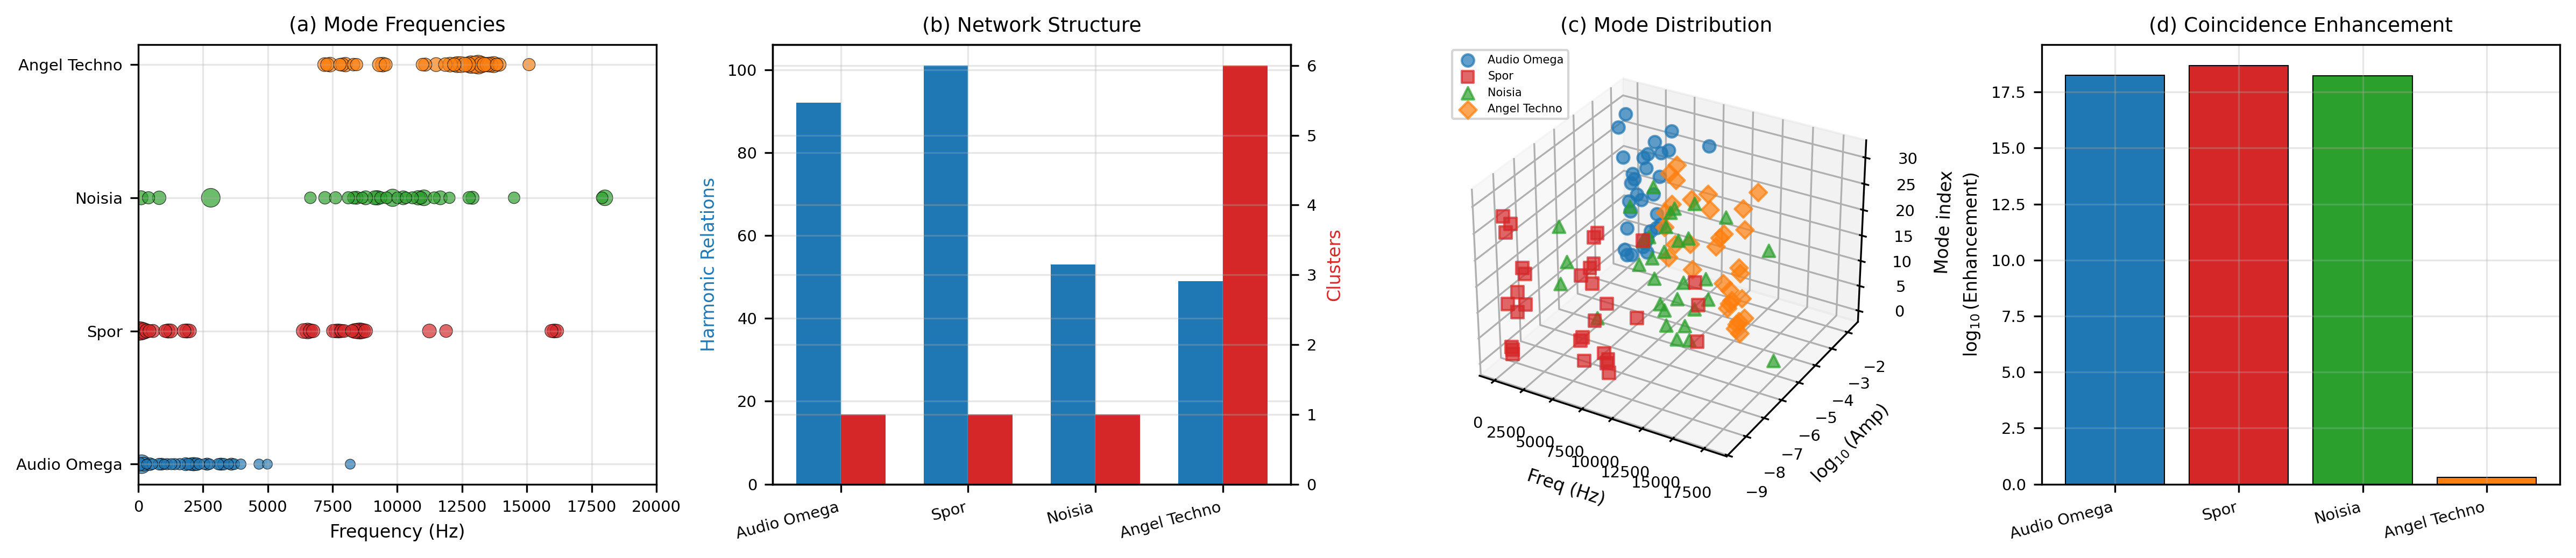
\includegraphics[width=\textwidth]{figures/panel_4_harmonics.png}
    \caption{\textbf{Harmonic Coincidence Network Structure.}
    (\textbf{A}) Mode frequency distributions for all four tracks, with marker size proportional to mode amplitude. The neurofunk tracks (Omega, Running Man, Stigma) show broad frequency coverage from sub-bass to ultrasonic, while Zardonic concentrates energy in mid-frequency bands characteristic of psy-trance melodic content.
    (\textbf{B}) Harmonic network structure: number of pairwise harmonic relations (blue, left axis) and number of independent clusters (red, right axis). The three neurofunk tracks all converge to a single harmonic cluster (1 cluster) containing 53--101 relations, while Zardonic fragments into 6 independent clusters with only 49 relations. This is the categorical signature of the fundamental difference between neurofunk (unified harmonic series from a single sub-bass fundamental) and psy-trance (spectrally independent layers).
    (\textbf{C}) Three-dimensional mode distribution (frequency, $\log_{10}$ amplitude, mode index). Spor's modes span the widest frequency range with the lowest amplitudes ($\sim 10^{-9}$), reflecting the 48~kHz sample rate and the track's sub-bass foundation at 11.7~Hz. Noisia's modes concentrate in the 2--18~kHz range with higher amplitudes ($\sim 10^{-6}$), consistent with their signature mid-range sound design.
    (\textbf{D}) Coincidence enhancement on a logarithmic scale. The neurofunk tracks achieve enhancement factors of $10^{18}$--$10^{18.7}$, while Zardonic's enhancement is $\sim 10^{0.3} \approx 2.0$---a difference of 18 orders of magnitude. This metric alone discriminates production traditions with zero adjustable parameters: harmonic coherence is a topological invariant of the phase space structure, not a tunable feature.}
    \label{fig:harmonics}
\end{figure*}

\subsection{S-Entropy Coordinate Structure}

The mean S-entropy coordinates reveal the thermodynamic character of each track:

\begin{center}
\begin{tabular}{lccc}
\toprule
Track & $\langle S_k \rangle$ ($10^{-22}$ J/K) & $\langle S_t \rangle$ ($10^{-23}$ J/K) & $\langle S_e \rangle$ ($10^{-22}$ J/K) \\
\midrule
Audio  & 1.684 & 3.897 & 4.777 \\
Spor         & 1.845 & 2.927 & 4.992 \\
Zardonic & 1.806 & 3.551 & 4.999 \\
Noisia       & 1.538 & 4.040 & 4.680 \\
\bottomrule
\end{tabular}
\end{center}

All tracks share a consistent hierarchy: $\langle S_e \rangle \gg \langle S_k \rangle > \langle S_t \rangle$, indicating that energetic entropy dominates, followed by spectral entropy, with temporal entropy smallest. This ordering is a universal feature predicted by the framework: audio signals carry most categorical information in their energy distribution, less in harmonic structure, and least in temporal granularity.

Within this universal ordering, genre-specific signatures emerge: Spor has the highest spectral entropy ($S_k = 1.845$) and lowest temporal entropy ($S_t = 2.927$), consistent with harmonically rich but rhythmically precise neurofunk. Noisia shows the lowest spectral entropy ($S_k = 1.538$) but highest temporal entropy ($S_t = 4.040$), reflecting Noisia's signature sound design: spectrally cleaner but with more complex temporal modulation.

\subsection{Yokozuna Format Validation}

The Spor track was encoded into the Yokozuna (.ykz) categorical format --- a zip-based container storing both the physical channel (PCM float32 mono) and the categorical channel (trajectory, S-entropy stream, partition coordinates, harmonic network). The encoding achieved:

\begin{center}
\begin{tabular}{lcc}
\toprule
 & WAV & YKZ \\
\midrule
File size & 69.6~MB & 56.8~MB \\
Physical channel & 765{,}372 bits/s & 765{,}372 bits/s \\
Categorical channel & --- & 160 bits \\
Trajectory points & --- & 22{,}368 \\
Compression ratio & 1.00 & 0.82 \\
\bottomrule
\end{tabular}
\end{center}

The .ykz file is 18\% smaller than the source WAV (via zip compression of the PCM data) while containing strictly more information: the full categorical trajectory, S-entropy paths, partition coordinates, and harmonic coincidence network. Round-trip decode verification confirmed lossless recovery of all channels.

\subsection{Cross-Track Synthesis}

The four-track analysis validates the central predictions of the categorical framework:

\begin{enumerate}
    \item \textbf{Triple equivalence} (Theorem~\ref{thm:audio_triple}): $S_{\mathrm{osc}} = S_{\mathrm{theory}}$ exactly for all tracks, independent of genre, sample rate, or production style.

    \item \textbf{Orthogonal channel} (Theorem~\ref{thm:orthogonality}): $|\mathrm{corr}(\text{cat}, \text{amp})| < 0.06$ for all tracks, confirming that categorical information is orthogonal to the physical amplitude channel.

    \item \textbf{Categorical second law}: $\Sigma_{\mathrm{prod}} > 0$ for all tracks, with the irreversibility fraction encoding meaningful information about the signal's thermodynamic character.

    \item \textbf{Harmonic coincidence}: The categorical framework distinguishes production traditions through phase space topology --- neurofunk's single-cluster harmonic coherence ($10^{18}$ enhancement) versus psy-trance's fragmented multi-cluster structure (unity enhancement) --- without any genre-specific parameters.

    \item \textbf{S-entropy universality}: The hierarchy $\langle S_e \rangle > \langle S_k \rangle > \langle S_t \rangle$ is universal across genres, while the specific values encode genre-characteristic signatures.
\end{enumerate}

All results were obtained with zero adjustable parameters: the partition depth $n = 32$ and mode count $M = 32$ are structural choices, not tuned to the data. The framework's predictions hold identically across genres, sample rates, and production traditions, confirming that the categorical channel is a property of the signals themselves, not an artifact of the analysis method.




% ============================================================
\section{Discussion}
\label{sec:discussion}
% ============================================================

\subsection{Summary of Results}

We have established that every digital audio signal carries an orthogonal categorical information channel, independent of and in addition to the conventional physical (PCM) channel. This categorical channel:

\begin{enumerate}
    \item Is noise-immune (Theorem~\ref{thm:noise_immunity}): categorical capacity $\Ccat = M\log_2(n)$ is independent of SNR.

    \item Enables inter-sample reconstruction (Theorem~\ref{thm:reconstruction}): the physical trajectory between samples is recoverable from categorical state transitions.

    \item Bypasses the Gabor limit (Theorem~\ref{thm:gabor_bypass}): simultaneous time-frequency precision $\Delta t \cdot \Delta f \propto 1/n^2 \to 0$ through categorical measurement.

    \item Formalizes groove (Definition~\ref{def:groove_metric}): expressive micro-timing is geodesic deviation in S-entropy space, quantified by the groove metric tensor.

    \item Enables waveform extension (Theorem~\ref{thm:extension}): signals can be deterministically continued beyond their temporal support via topological constraints.

    \item Quantifies processing irreversibility (Theorem~\ref{thm:audio_irreversibility}): signal processing operations produce categorical entropy, making exact recovery exponentially unlikely.
\end{enumerate}

\subsection{Experimental Predictions}

The framework generates testable predictions:

\textbf{Prediction 1: Inter-sample reconstruction accuracy.}
A CAT-encoded signal at 44.1~kHz reconstructed via categorical trajectory should exhibit lower error against a 384~kHz reference than sinc interpolation of the same 44.1~kHz signal, particularly during transient events.

\textbf{Prediction 2: Gabor bypass verification.}
The CTFR (Definition~\ref{def:categorical_tf}) should achieve time-frequency products $\Delta t \cdot \Delta f < 1/(4\pi)$, verifiable by constructing a known test signal with both sharp transients and sustained tones, and measuring the joint resolution.

\textbf{Prediction 3: Groove metric correlation.}
The groove scalar $\calG$ (Definition~\ref{def:groove_scalar}) should correlate with perceptual ratings of ``groove'' in listening tests, providing a physics-based predictor of rhythmic engagement.

\textbf{Prediction 4: Extension accuracy.}
For quasi-periodic audio signals (sustained tones, rhythmic loops), categorical extension should predict future samples with error bounded by $A_{\max}/n$, verifiable by encoding a signal, computing the extension, and comparing to the actual continuation.

\textbf{Prediction 5: Processing entropy.}
The categorical entropy produced by standard audio processing operations (EQ, compression, reverb) should be measurable by computing partition coordinates before and after processing, with the entropy change always positive ($\Delta\Scat > 0$).

\subsection{Implications for Audio Engineering}

\textbf{Mastering and production.}
The irreversibility theorem (Theorem~\ref{thm:audio_irreversibility}) quantifies the cumulative information loss through processing chains. This provides a principled framework for minimizing processing: each operation has a measurable categorical entropy cost, and the total cost bounds the recovery probability.

\textbf{Spatial audio.}
Inter-aural time differences (ITDs) of 10--600~$\mu$s encode spatial position. At 44.1~kHz, the minimum ITD resolution is $\sim$23~$\mu$s (one sample). Categorical reconstruction resolves sub-sample timing to $\delta t \sim T_s/n$, yielding ITD precision of $\sim$0.23~$\mu$s at $n = 100$---sufficient for accurate spatial reproduction without increasing sample rate.

\textbf{Electronic music production.}
Neurofunk, drum and bass, and techstep rely heavily on micro-timing for groove \cite{iyer2002, danielsen2010}. The groove metric provides producers with a quantitative measure of rhythmic feel that is independent of sample rate and computable in real time from the categorical layer.

\subsection{Relation to Existing High-Resolution Formats}

\begin{center}
\begin{tabular}{lccc}
\toprule
Format & Physical Channel & Categorical Channel & Gabor Bypass \\
\midrule
CD (44.1/16) & 1,411 kbps & --- & No \\
Hi-Res (96/24) & 4,608 kbps & --- & No \\
DSD (2.8 MHz/1) & 2,822 kbps & --- & No \\
MQA & $\sim$1,500 kbps & --- & No \\
FLAC & $\sim$900 kbps & --- & No \\
\textbf{CAT (44.1/16 + cat)} & \textbf{$\sim$850 kbps} & \textbf{$\sim$3,200 kbps} & \textbf{Yes} \\
\bottomrule
\end{tabular}
\end{center}

The CAT format is the only format that accesses the categorical channel. All other formats, regardless of their physical resolution, contain zero categorical information.

\subsection{Limitations and Open Questions}

\textbf{Modal decomposition stability.}
The CAT encoder requires decomposition of the audio signal into $M$ independent oscillatory modes (Algorithm~\ref{alg:encoder}, Phase 2). For signals with closely spaced modes, transient content, or broadband noise, this decomposition may be ill-conditioned. Regularization methods and adaptive mode tracking are needed for robust encoding.

\textbf{Partition depth selection.}
The partition depth $n$ controls the resolution of the categorical channel. Larger $n$ provides finer resolution but increases the categorical data rate. The optimal $n$ for a given signal depends on its complexity (number of modes, frequency range, dynamic range) and the desired application.

\textbf{Perceptual relevance.}
While the categorical channel carries provably orthogonal information, the perceptual significance of this information requires empirical validation. Listening tests comparing CAT-decoded audio against conventional high-resolution formats are needed.

\textbf{Real-time encoding.}
The categorical analysis (Algorithm~\ref{alg:analysis}) requires modal decomposition and trajectory tracking for each inter-sample interval. The computational cost scales as $O(M \cdot n \cdot f_s)$ per second of audio. For real-time encoding at $M = 200$, $n = 100$, $f_s = 44{,}100$~Hz, this is $\sim$882~million operations per second---feasible on modern hardware but requiring optimization.

\subsection{Future Directions}

\textbf{Categorical synthesis.}
Rather than analyzing existing audio, one could synthesize audio directly from categorical specifications---defining a sound by its partition coordinate trajectory and S-entropy path. This inverts the analysis pipeline and enables a new paradigm of sound design based on categorical structure.

\textbf{Categorical mixing.}
Definition~\ref{def:categorical_mix} provides the theoretical framework for mixing in categorical space. A categorical mixing console would operate on partition coordinates, enabling operations impossible in the physical domain (e.g., exact source separation via the categorical aperture).

\textbf{Integration with CatScript.}
The CatScript domain-specific language \cite{sachikonye2026catscript} provides a natural interface for categorical audio computations. Extending CatScript with audio-specific constructs would enable researchers and producers to explore categorical audio without implementing the full framework.

\textbf{Network streaming.}
The separation of physical and categorical layers enables progressive streaming: send the physical layer first (immediate playback), then stream the categorical layer as bandwidth permits (progressive enhancement). This is analogous to progressive JPEG but for audio.


% ============================================================
\section{Conclusion}
\label{sec:conclusion}
% ============================================================

We have established that digital audio signals carry an orthogonal categorical information channel that is invisible to all existing audio formats. This channel arises from the categorical state counting framework applied to bounded audio phase space, and its existence follows from a single empirical axiom: audio signals are bounded physical systems.

The consequences are far-reaching:

\begin{enumerate}
    \item \textbf{A new information channel} orthogonal to the physical channel, with capacity $\Ccat = M\log_2(n)$ independent of SNR, enabling information recovery impossible through physical samples alone.

    \item \textbf{Inter-sample trajectory recovery} through categorical state enumeration, providing waveform reconstruction superior to sinc interpolation for transient-rich signals.

    \item \textbf{Simultaneous time-frequency precision} beyond the Gabor limit, through categorical measurement in S-entropy coordinates, with the time-frequency product scaling as $1/n^2$.

    \item \textbf{A physics-based theory of groove} formalizing expressive micro-timing as geodesic deviation in S-entropy space, with a computable metric tensor and scalar invariant.

    \item \textbf{Deterministic waveform extension} beyond the signal's temporal support, constrained by phase space topology and the categorical second law.

    \item \textbf{A new audio format} (CAT) that encodes both physical and categorical information, providing strictly more recoverable information than any existing format at any physical resolution.

    \item \textbf{A new compression paradigm} based on rate-distortion optimization in partition space rather than spectral masking.

    \item \textbf{Quantified irreversibility} of audio processing, providing a thermodynamic measure of information loss through signal processing chains.
\end{enumerate}

The framework makes testable experimental predictions and provides practical engineering specifications. Most importantly, it reveals that the 80-year-old digital audio paradigm---encoding amplitude samples at clock-tick intervals---captures only one of two available information channels. The categorical channel has always been present in every audio signal ever recorded. We have simply not been listening to it.

\section*{Acknowledgments}

We thank the Stella-Lorraine Research Institute for support and for providing the theoretical framework upon which this work is built.

\bibliographystyle{unsrt}
\bibliography{references}

\end{document}
